\documentclass[11pt]{article}

% Shared preamble and notation for the numerical Einstein equations article.

\usepackage[utf8]{inputenc}
\usepackage[T1]{fontenc}
\usepackage{amsmath}
\usepackage{amssymb}
\usepackage{amsfonts}
\usepackage{amsthm}
\usepackage{mathtools}
\usepackage{mathrsfs}
\usepackage{bm}
\usepackage{booktabs}
\usepackage{array}
\usepackage{enumitem}
\usepackage{graphicx}
\usepackage[dvipsnames]{xcolor}
\usepackage[final,expansion=false]{microtype}
\usepackage[a4paper,top=2.5cm,bottom=2.5cm,left=3cm,right=3cm]{geometry}
\usepackage[colorlinks=true,linkcolor=MidnightBlue,citecolor=MidnightBlue,
            urlcolor=MidnightBlue]{hyperref}

\allowdisplaybreaks
\numberwithin{equation}{section}
\setlist[enumerate]{leftmargin=*,itemsep=0.4em}
\setlist[itemize]{leftmargin=*,itemsep=0.25em}

\theoremstyle{plain}
\newtheorem{theorem}{Theorem}[section]
\newtheorem{proposition}[theorem]{Proposition}
\newtheorem{lemma}[theorem]{Lemma}
\newtheorem{corollary}[theorem]{Corollary}

\theoremstyle{definition}
\newtheorem{definition}[theorem]{Definition}
\newtheorem{experiment}[theorem]{Experiment}

\theoremstyle{remark}
\newtheorem{remark}[theorem]{Remark}

\newcommand{\R}{\mathbb R}
\newcommand{\C}{\mathbb C}
\newcommand{\Z}{\mathbb Z}
\newcommand{\Sph}{\mathbb S^2}
\newcommand{\dd}{\mathop{}\!\mathrm d}
\newcommand{\pd}{\partial}
\newcommand{\Lie}{\mathcal L}
\newcommand{\Rc}{\operatorname{Ric}}
\newcommand{\Riem}{\operatorname{Riem}}
\newcommand{\tr}{\operatorname{tr}}
\newcommand{\tf}{\operatorname{tf}}
\newcommand{\diver}{\operatorname{div}}
\newcommand{\curl}{\operatorname{curl}}
\newcommand{\Sym}{\operatorname{Sym}}
\newcommand{\Boxg}{\Box_{\mathbf g}}
\newcommand{\norm}[1]{\left\lVert #1\right\rVert}
\newcommand{\abs}[1]{\left\lvert #1\right\rvert}
\newcommand{\inner}[2]{\left\langle #1,#2\right\rangle}
\newcommand{\restr}[2]{\left.#1\right|_{#2}}

\newcommand{\bg}{\mathbf g}
\newcommand{\slg}{\gamma}
\newcommand{\roundg}{\overset{\circ}{\gamma}}
\newcommand{\sK}{K}
\newcommand{\sRic}{Ric\mkern-19mu /\,\,\,\,}
\newcommand{\sL}{{\cal L}\mkern-10mu /}
\newcommand{\sLh}{\hat{\sL}}
\newcommand{\sg}{g\mkern-9mu /}
\newcommand{\seps}{\epsilon\mkern-8mu /}
\newcommand{\sd}{d\mkern-10mu /}
\newcommand{\sR}{R\mkern-10mu /}
\newcommand{\snab}{\nabla\mkern-13mu /\,\,}
\newcommand{\sdiv}{\mbox{div}\mkern-19mu /\,\,\,\,}
\newcommand{\scurl}{\mbox{curl}\mkern-19mu /\,\,\,\,}
\newcommand{\strc}{\mbox{tr}\mkern-13mu /\,\,}
\newcommand{\slap}{\mbox{$\triangle  \mkern-13mu / \,$}}
\newcommand{\Hb}{\underline H}
\newcommand{\Lb}{\underline L}
\newcommand{\chib}{\underline\chi}
\newcommand{\chih}{\widehat\chi}
\newcommand{\chibh}{\widehat{\underline\chi}}
\newcommand{\etab}{\underline\eta}
\newcommand{\omegab}{\underline\omega}
\newcommand{\alphab}{\underline\alpha}
\newcommand{\betab}{\underline\beta}
\newcommand{\hatotimes}{\mathbin{\widehat\otimes}}

\newcommand{\Aout}{A}
\newcommand{\Ain}{\underline A}
\newcommand{\Xout}{\mathcal X}
\newcommand{\Xin}{\underline{\mathcal X}}
\newcommand{\Sigmaout}{\Sigma}
\newcommand{\Sigmain}{\underline\Sigma}
\newcommand{\Wout}{W}
\newcommand{\Win}{\underline W}
\newcommand{\Pthree}{P}
\newcommand{\Pfour}{Q}
\newcommand{\Gradphi}{\Pi}

\newcommand{\State}{\mathcal U}
\newcommand{\BoundaryData}{\mathcal D}
\newcommand{\Config}{\mathcal C}
\newcommand{\Picard}{\Phi}
\newcommand{\Domain}{\mathcal Q}
\newcommand{\Proj}{\Pi}
\newcommand{\Residual}{\mathfrak R}
\newcommand{\Defect}{\mathfrak D}
\newcommand{\diag}{\operatorname{diag}}
\newcommand{\eps}{\varepsilon}
\newcommand{\dv}{\operatorname{div}}
\newcommand{\cl}{\operatorname{curl}}

\def\oc{\overset{\circ}}
\def\wt{\widetilde}

\hypersetup{
  pdftitle={Picard Iteration for the Characteristic Initial Value Problem in Einstein Equations},
  pdfauthor={Shengrong Wu}
}

\title{Picard Iteration for the Characteristic Initial Value Problem in Einstein Equations}
\author{Shengrong Wu}
\date{\today}

\begin{document}

\maketitle
\begin{abstract}
    We present an iteration algorithm for vacuum and
    Einstein scalar-field equations in double-null gauge, which transform the non-linear PDE into systems of ODE. The numerical
    realization combines characteristic constraint solves, LGL spectral
    elements, pole-free spherical operators, Galerkin projection, and
    independent geometric residual audits.
\end{abstract}
\tableofcontents

\section{Introduction}

The characteristic initial value problem is a natural formulation of the
Einstein equations when radiation, null focusing, and the formation of
trapped surfaces are central.  Instead of prescribing data on a spacelike
hypersurface, one prescribes compatible data on two intersecting null
hypersurfaces and evolves their future domain of dependence.  Local
well-posedness for this problem is known under suitable regularity
assumptions~\cite{rendall-90,luk-12,cabet-16,hilditch-20}, but its direct
numerical realization becomes substantially more difficult once spherical
symmetry is removed.  The use of null hypersurfaces as an evolution framework
goes back to the Bondi--Sachs description of gravitational radiation and the
early analysis of characteristic data~\cite{bondi-62,sachs-civp-62}; its
development as a numerical method is surveyed in~\cite{winicour-12}.

Characteristic numerical relativity has progressed from double-null vacuum
evolutions with two Killing symmetries~\cite{corkill-stewart-83} and
spherically symmetric scalar collapse in null coordinates
~\cite{garfinkle-95,hamade-stewart-96} to axisymmetric vacuum evolution on
outgoing null cones~\cite{gomez-94} and generic angular data for accurate
Cauchy--characteristic waveform extraction~\cite{moxon-23}.  Numerical
relativity has also long evolved nonspherical spacetimes in spacelike
foliations.  Fully three-dimensional Cauchy calculations have studied
scalar-field collapse without symmetry assumptions~\cite{deppe-19}, and
axisymmetric pseudospectral calculations have reached strongly aspherical
regimes in which the center of collapse bifurcates~\cite{marouda-24}.  The
first null-coordinate simulations of nonspherical regular data collapsing
to a black hole were obtained in twist-free axisymmetry for the massless
scalar field~\cite{gundlach-24}; that work describes the accessible data as
moderately nonspherical and identifies larger deviations from spherical
symmetry, as well as vacuum collapse, as important challenges.  Thus the gap
addressed here is not an absence of nonspherical numerical solutions in
general.  It is the relative scarcity of direct characteristic evolutions
with strongly nonspherical, freely prescribed initial geometry in a fully
angular double-null gauge.

Let $(u,v,\theta^A)$ be double-null coordinates.  We write the spacetime
metric as
\begin{equation}\label{eq:introduction-double-null-metric}
  \bg=-2\Omega^2(\dd u\otimes\dd v+\dd v\otimes\dd u)
  +g_{AB}(\dd\theta^A-b^A\dd u)\otimes
   (\dd\theta^B-b^B\dd u).
\end{equation}
The metric is therefore represented by the section metric $g_{AB}$, the
lapse $\Omega$, and the angular shift $b$.  This formulation gives
considerable freedom to choose the geometry on the two initial null
hypersurfaces, subject to the characteristic constraints and corner
compatibility.  In particular, the nonspherical part of the initial metric
variation can be prescribed directly rather than produced only indirectly
from a matter perturbation or a spacelike constraint solve.  The fourth
experiment gives a quantitatively strong example: on its outgoing initial
hypersurface, where $\Omega=1$, the prescribed data satisfy
\begin{equation}\label{eq:introduction-strong-asymmetry}
  \norm{\tf\Lie_{\partial_v}g(-1,0.005)}_{L^2(S)}=7.50960,
  \qquad
  \norm{\tf\Lie_{\partial_v}g(-1,0.005)}_{L^\infty(S)}=2.53468.
\end{equation}
The perturbation is consequently a substantial geometric departure from
spherical symmetry, rather than a nonspherical profile whose effect on the
initial metric is numerically negligible.

This paper develops a first-order Picard iteration for both the Einstein
vacuum equations
\begin{equation}
  \Rc(\bg)=0
\end{equation}
and the Einstein--massless-scalar system
\begin{equation}
  \Rc(\bg)=\dd\phi\otimes\dd\phi,
  \qquad \Boxg\phi=0,
\end{equation}
in the gauge \eqref{eq:introduction-double-null-metric}.  The iteration is
organized by the geometry of the characteristic problem.  Data that are
free, data fixed by the null constraints, and quantities transported in the
two characteristic directions play different roles in each sweep.  The
resulting construction is therefore not obtained by treating all coordinate
components as an undifferentiated system of equations: its update order
follows the causal and geometric dependency structure of the double-null
equations.

Two difficulties are particularly important.  The first is to obtain an
executable form of the equations.  Analytic arguments can often group
lower-order terms schematically or pass between conventionally equivalent
forms, whereas numerical evolution requires every displayed sign and
numerical factor to be fixed consistently.  We address this by checking the
formulas against identities derived from the four-metric, by testing exact
solutions, and by evaluating curvature residuals independently of the
quantities used to construct a Picard sweep.  The second difficulty is the
iteration itself.  Its design requires identifying a closed hierarchy that
respects the characteristic constraints, transports information in the
correct direction, preserves the two initial traces, and remains meaningful
as the null hypersurfaces focus.  This construction comes from the geometric
structure of the equations rather than from a generic fixed-point template.

The numerical implementation combines Legendre--Gauss--Lobatto spectral
elements in the two null coordinates with pole-free spherical
differentiation, angular Galerkin projection, characteristic constraint
solves, and independent overgrid audits.  Extensive AI-assisted software
development made it practical to implement, refactor, and test this large
coupled system.  The mathematical conventions, iteration design, experiment
definitions, acceptance criteria, and scientific interpretation remain
author-controlled; confidence in the computations is based on exact
benchmarks, convergence studies, immutable characteristic data, and
independent residual evaluation rather than on code generation itself.

Eight numerical experiments test complementary aspects of the method.  The
exact-solution tests cover Schwarzschild, Kerr, and Fisher--JNW spacetimes.
They measure the metric error in regular regions, across a Schwarzschild
horizon, and toward a curvature singularity.  The vacuum experiments evolve a
strong nonspherical outgoing perturbation and crossed characteristic data
whose initial curvature is singular at the corner.  The final experiments
evolve nonspherical Einstein--scalar data and a stronger scalar pulse toward
a trapped region.  In the last experiment, an inner atlas of characteristic
rectangles covers a curved domain adapted to null focusing.  Independent
four-metric evaluation finds the section
\begin{equation}\label{eq:introduction-trapped-section}
  (u,v)=(-0.4696271025,0.04)
\end{equation}
on which the two future null expansions are strictly negative everywhere,
with respective spherical suprema $-0.0802152$ and $-4.28011$.  Solving the
angular marginally outer trapped surface equation on successive incoming
null cones then reconstructs an apparent-horizon tube of 18 sections over
$0.00441\leq v\leq0.05$.  Coordinate and angular controls agree on its
$v=0.04$ section to better than $1.6\times10^{-7}$ in the graph location.

This trapped-section computation is motivated by An's proof that anisotropic
outgoing characteristic perturbations of Christodoulou's naked-singularity
data generate an anisotropic apparent horizon that censors the
singularity~\cite{an-25}.  The numerical experiment does not constitute a
proof of that theorem, and the reconstructed tube is tied to the chosen
incoming-null foliation.  It does, however, provide a coordinate- and
angularly controlled numerical realization of the associated trapped-region
mechanism and its anisotropic apparent horizon.

Section~2 fixes the double-null equations and records the analytic framework.
Section~3 constructs the Picard map and its numerical discretization.
Sections~4 and~5 present the vacuum and Einstein--scalar experiments,
respectively, and distinguish exact metric errors from independently
evaluated curvature residuals.


\section{Equations and Theoretical Analysis}
\subsection{Double null foliation and equations}
In this section, we introduce the equations for Lorentzian metric under double null foliation. Let $(\mathcal{M},g)$ be a $4$-dimensional Lorentzian manifold. With double null coordinates $(u,v,\theta^A)$, the metric can be written as 
\begin{equation}
    g=-2\Omega^2(du\otimes dv+dv\otimes du)+g_{AB}(d\theta^A-b^Adu)\otimes (d\theta^B-b^Bdu),
\end{equation}
and we use $(g_{AB},b^A,\Omega)$ to represent the metric. The level sets of $u$ and $v$ are denoted by $H_u$ and $\Hb_{v}$ respectively, and their spherical intersection $H_u\cap\Hb_v$ is denoted by $S_{u,v}$.
With double null frame 
\[e_3=\Omega^{-1}(\partial_u+b),\ e_4=\Omega^{-1}\partial_v,\ e_A=\partial_{\theta^A},\]
we can define Ricci coefficients, or connection components
\begin{equation}\label{Ricci_coefficients_definition}
    \begin{aligned}
    \chi_{A B}=g\left(D_A e_4, e_B\right), &\qquad \underline{\chi}_{A B}=g\left(D_A e_3, e_B\right), \\
    \eta_A=-\frac{1}{2} g\left(D_3 e_A, e_4\right), &\qquad \underline{\eta}_A=-\frac{1}{2} g\left(D_4 e_A, e_3\right), \\
    {\omega}=-\frac{1}{4} g\left(D_4 e_3, e_4\right), &\qquad \underline{\omega}=-\frac{1}{4} g\left(D_3 e_4, e_3\right),\\
    \zeta_A=\frac{1}{2}g\left(D_A e_4,e_3\right)&=-\frac{1}{4}\Omega^{-2}(\Lie_vb^B)g_{AB}.
    \end{aligned}
\end{equation}
Their transport equations are listed below:
\begin{equation}\label{eq:Ricci_coefficients_propagation_1}
    \begin{aligned}
        \nabla_4 \operatorname{tr} \chi+\frac{1}{2}(\operatorname{tr} \chi)^2=&-\operatorname{Ric}_{44}-|\hat{\chi}|^2-2 \omega \operatorname{tr} \chi, \\
     \nabla_3 \operatorname{tr} \underline{\chi}+\frac{1}{2}(\operatorname{tr} \underline{\chi})^2=&-\operatorname{Ric}_{33}-|\underline{\hat{\chi}}|^2-2 \underline{\omega} \operatorname{tr} \underline{\chi},
    \end{aligned}
\end{equation}
\begin{equation}\label{eq:Ricci_coefficients_propagation_2}
    \begin{aligned}
        \nabla_3 \hat{\chi}_{A B}+\frac{1}{2} \operatorname{tr} \underline{\chi} \hat{\chi}_{A B}=&\widehat{\operatorname{Ric}}_{A B}+2 \underline{\omega} \hat{\chi}_{A B}+(\snab  \hat{\otimes} \eta)_{A B}+(\eta \hat{\otimes} \eta)_{A B}-\frac{1}{2} \operatorname{tr} \chi \underline{\hat{\chi}}_{A B}, \\
     \nabla_4 \underline{\hat{\chi}}_{A B}+\frac{1}{2} \operatorname{tr} \chi \underline{\hat{\chi}}_{A B}=&\widehat{\operatorname{Ric}}_{A B}+2 \omega \underline{\hat{\chi}}_{A B}+(\snab\hat{\otimes} \underline{\eta})_{A B}+(\underline{\eta} {\hat{\otimes}} \underline{\eta})_{A B}-\frac{1}{2} \operatorname{tr} \underline{\chi} \hat{\chi}_{A B},
    \end{aligned}
\end{equation}
\begin{equation}
    \begin{aligned}
        \nabla_3 \operatorname{tr} \chi=&-\frac{1}{2} \operatorname{tr} \chi \operatorname{tr} \underline{\chi}+\sg^{A B} R_{3 A B 4}+2 \underline{\omega} \operatorname{tr} \chi+2 \sdiv \eta+2|\eta|^2-\hat{\chi} \cdot \underline{\hat{\chi}}\\
        =&-\tr\chi\tr\chib+2\omegab\tr\chi+2\sdiv\eta+2\left|\eta\right|^2-2K+R+\Rc_{34}, \\
        \nabla_4 \operatorname{tr} \underline{\chi}=&-\frac{1}{2} \operatorname{tr} \chi \operatorname{tr} \underline{\chi}+\sg^{A B} R_{3 A B 4}+2 \omega \operatorname{tr} \underline{\chi}+2 \sdiv \underline{\eta}+2|\underline{\eta}|^2-\hat{\chi} \cdot \underline{\hat{\chi}}\\
        =&-\tr\chi\tr\chib+2\omega\tr\chib+2\sdiv\etab+2\left|\etab\right|^2-2K+R+\Rc_{34}.
    \end{aligned}
\end{equation} 
\begin{equation}\label{eq:Ricci_coefficients_propagation_3}
    \begin{aligned}
        \nabla_4 \eta=&-\chi \cdot(\eta-\underline{\eta})-\frac{1}{2} R_{A 434}, \\
        \nabla_3 \underline{\eta}=&-\underline{\chi} \cdot(\underline{\eta}-\eta)-\frac{1}{2} R_{A 343}, \\
        \nabla_4 \underline{\omega}=&\frac{1}{4}\left(\operatorname{Ric}_{34}+\sg^{A B} R_{3 A B 4}\right)+2 \underline{\omega} \omega+\frac{1}{2}|\eta|^2-\eta \cdot \underline{\eta}\\
        =&2\omega\omegab-\frac{1}{2}  K+\frac{1}{2} \Rc_{34}+\frac{1}{4} R +\frac{1}{4}\chih\cdot\chibh-\frac{1}{8}\tr\chi\,\tr\chib+\frac{1}{2}\left|\eta\right|^2-\eta\cdot\etab, \\
        \nabla_3 \omega=&\frac{1}{4}\left(\operatorname{Ric}_{34}+\sg^{A B} R_{3 A B 4}\right)+2 \underline{\omega} \omega+\frac{1}{2}|\underline{\eta}|^2-\eta \cdot \underline{\eta}\\
        =&2\omega\omegab-\frac{1}{2}  K+\frac{1}{2} \Rc_{34}+\frac{1}{4} R +\frac{1}{4}\chih\cdot\chibh-\frac{1}{8}\tr\chi\,\tr\chib+\frac{1}{2}\left|\underline\eta\right|^2-\eta\cdot\etab.
    \end{aligned}
\end{equation}
Moreover, we have equations for $\zeta$:
\begin{equation}\label{eq:Ricci_coefficients_propagation_4}
    \begin{aligned}
        &\Omega\Rc_{3A}=\Omega\nabla_3\zeta+\frac{3}{2}\Omega\tr\chib\zeta+\Omega\chibh\cdot\zeta+\Omega\tr\chib\nabla\log\Omega\\
        &\qquad\qquad\qquad+2\nabla(\Omega\omegab)+\dv(\Omega\chibh)-\frac{1}{2}\nabla(\Omega\tr\chib),\\
        &\Omega\Rc_{4A}=-\Omega\nabla_4\zeta-\frac{3}{2}\Omega\tr\chi\zeta-\Omega\chih\cdot\zeta+\Omega\tr\chi\nabla\log\Omega\\
        &\qquad\qquad\qquad+2\nabla(\Omega\omega)+\dv(\Omega\chih)-\frac{1}{2}\nabla(\Omega\tr\chi).
    \end{aligned}
\end{equation}
Here $K$ stands for Gaussian curvature of topological sphere $S_{u,v}$. Gauss-Codazzi equations imply 
\begin{equation}\label{eq:Gauss-Codazzi_1}
        \begin{aligned}
         K=&\frac{1}{2} \sg^{A B} R_{3 A 4 B}+\frac{1}{2} R+\frac{1}{2} \operatorname{Ric}_{34}+\frac{1}{2} \hat{\chi} \cdot \underline{\hat{\chi}}-\frac{1}{4} \operatorname{tr} \chi \operatorname{tr} \underline{\chi}, 
        \end{aligned}
        \end{equation}
\begin{equation}\label{eq:Gauss-Codazzi_2}
            \begin{aligned} 
            \snab^B \hat{\chi}_{A B}-\frac{1}{2} \snab_A \operatorname{tr} \chi=&-\frac{1}{2} R_{A 434}+\operatorname{Ric}_{4 A}+\frac{1}{2} \operatorname{tr} \chi \zeta_A-\zeta^B \hat{\chi}_{A B}, \\
            \snab^B \underline{\hat{\chi}}_{A B}-\frac{1}{2} \snab_A \operatorname{tr} \underline{\chi}=&-\frac{1}{2} R_{A 343}+\operatorname{Ric}_{3 A}-\frac{1}{2} \operatorname{tr} \underline{\chi} \zeta_A+\zeta^B \underline{\hat{\chi}}_{A B}.
            \end{aligned}
        \end{equation}
\begin{equation}\label{eq:curl-eta-etab}
            \begin{aligned}
                \snab_A \eta_B-\snab_B \eta_A=&R_{4[A B] 3}+\underline{\hat{\chi}}^C{ }_{[A} \hat{\chi}_{B] C}, \\
         \snab_A \underline{\eta}_B-\snab_B \underline{\eta}_A=&-R_{4[A B] 3}-\underline{\hat{\chi}}^C{ }_{[A} \hat{\chi}_{B] C}, \\
            \end{aligned}
        \end{equation}
For Weyl curvature,
\begin{equation*}
    W_{\mu\nu\theta\lambda}=R_{\mu\nu\theta\lambda}-\frac{1}{2}\left(\Rc_{\mu\theta}g_{\nu\lambda}+g_{\mu\theta}\Rc_{\nu\lambda}-\Rc_{\nu\theta}g_{\mu\lambda}-g_{\nu\theta}\Rc_{\mu\lambda}\right)+\frac{R}{6}\left(g_{\mu\theta}g_{\nu\lambda}-g_{\nu\theta}g_{\mu\lambda}\right),
\end{equation*}
we define the curvature components
\begin{equation}
\begin{aligned}
\beta_A & =\frac{1}{2} W\left(e_A, e_4, e_3, e_4\right), & & \underline{\beta}_A=\frac{1}{2} W\left(e_A, e_3, e_3, e_4\right), \\
\rho & =\frac{1}{4} W\left(e_4, e_3, e_4, e_3\right), & & \sigma=\frac{1}{4}{ }^* W\left(e_4, e_3, e_4, e_3\right).
\end{aligned}
\end{equation}
Then previous equations imply the following algebraic relations,
\begin{equation}
    K=-\rho+\frac{1}{2}R+\Rc_{34}+\frac{1}{2}\chibh\cdot\chih-\frac{1}{4}\tr\chib\tr\chi,
\end{equation}
\begin{equation}
    \cl\eta=-\cl\etab=\sigma+\frac{1}{2}\chibh\wedge\chih,
\end{equation}
\begin{equation}\label{Codazzi_eq_chi}
    \dv\chih-\frac{1}{2}\nabla\tr\chi=-\beta+\frac{1}{2}\Rc_{4\cdot}+\frac{1}{2}\tr\chi\zeta-\zeta\cdot\chih,
\end{equation}
\begin{equation}\label{Codazzi_eq_chib}
    \dv\chibh-\frac{1}{2}\nabla\tr\chib=\betab+\frac{1}{2}\Rc_{3\cdot}-\frac{1}{2}\tr\chib\zeta+\zeta\cdot\chibh.
\end{equation}
After introducing the reduced curvature
\begin{equation}
    \beta^r_A=\beta_A-\frac{1}{2}\Rc_{4A},\, \betab^r_A=\betab_A+\frac{1}{2}\Rc_{3A}, \,\sigma^r=\sigma+\frac{1}{2}\chibh\wedge\chih,
\end{equation}
we can write the equations for curvature components
\begin{equation}
    \begin{aligned}
        &\Omega\nabla_3 K+\Omega\tr\chib K=\dv \left(\Omega\betab^r\right)+\frac{1}{2}\dv\left(\eta\Omega\tr\chib\right)-\dv\left(\eta\cdot\Omega\chibh\right),\\
         &\Omega\nabla_4 K+\Omega\tr\chi K=-\dv \left(\Omega\beta^r\right)+\frac{1}{2}\dv\left(\etab\Omega\tr\chi\right)-\dv\left(\etab\cdot\Omega\chih\right),
    \end{aligned}
\end{equation}
\begin{equation}
    \begin{aligned}
        \nabla_3\beta^r&+\left(\tr\chib-2\omegab\right) \beta^r=-\nabla K+{}^*\nabla\sigma+2\chih\cdot\betab\\
        &\qquad+\frac{1}{2}\left(\nabla(\chih\cdot\chibh)-{}^*\nabla(\chih\wedge\chibh)\right)-\frac{1}{4}\nabla\left(\tr\chi\tr\chib\right)\\
        &\qquad+3(\eta\rho+{}^*\eta\sigma)+\nabla_A\left(g^{CD}\Rc_{CD}\right)-\nabla^B \Rc_{BA}-\frac{1}{2}\tr\chib \Rc_{4A},\\
        \nabla_4\betab^r&+\left(\tr\chi -2\omega\right)\betab^r=\nabla K+{}^*\nabla\sigma+2\chibh\cdot\beta\\
        &\qquad-\frac{1}{2}\left(\nabla(\chih\cdot\chibh)+{}^*\nabla(\chih\wedge\chibh)\right)+\frac{1}{4}\nabla\left(\tr\chi\tr\chib\right)\\
        &\qquad-3\left(\etab\rho-{}^*\etab\sigma\right) -\nabla_A(g^{CD}\Rc_{CD})+\nabla^B \Rc_{BA}+\frac{1}{2}\tr\chi \Rc_{3A}.
    \end{aligned}
\end{equation}
Using \eqref{eq:Ricci_coefficients_propagation_3}, we derive 
\begin{equation}
  \begin{aligned}
      \Omega\nabla_3\cl\etab+\Omega\tr\chib\cl\etab=&\cl(\Omega\betab^r)+\epsilon^{AC}\nabla_A\left(\Omega\chib\cdot\eta\right)_C-\epsilon^{AC}\nabla_A(\Omega\Rc)_{C3},\\
      \Omega\nabla_4\cl\eta+\Omega\tr\chi\cl\eta=&-\cl(\Omega\beta^r)+\epsilon^{AC}\nabla_A\left(\Omega\chi\cdot\etab\right)_C-\epsilon^{AC}\nabla_A(\Omega\Rc)_{C4},
  \end{aligned}
\end{equation}
and
\begin{equation}
    \begin{aligned}
        &\Omega\nabla_3\left(\dv \etab-K\right)+\Omega\tr\chib\left(\dv \etab-K\right)=4\dv(\Omega\chibh\cdot\zeta)-\dv(\Omega\Rc_3),\\
        &\Omega\nabla_4\left(\dv \eta-K\right)+\Omega\tr\chi\left(\dv \eta-K\right)=-4\dv(\Omega\chih\cdot\zeta)-\dv(\Omega\Rc_4).
    \end{aligned}
\end{equation}
For a scalar function $\phi$, there is equation
\begin{equation}\label{eq:ese-wave-eq}
    -\Omega^2\square\phi=\Omega e_3(\Omega e_4\phi)+\frac{1}{2}\Omega\tr\chi\Omega e_3\phi+\frac{1}{2}\Omega\tr\chib\Omega e_4\phi-\Omega^2\Delta\phi-2\Omega^2\eta\cdot\nabla\phi.
\end{equation}

\subsection{Local existence}
We now introduce some results on Einstein vacuum equations. Similar results can be derived for other Einstein field equations and we omit them due to length of the article.

We first state the existence theorem for characteristic initial value problem of Einstein vacuum equations from \cite{luk-12}.
\begin{theorem}
    Given initial null hypersurface $H_0,\Hb_0$ and regular initial metric $(g,\Omega,b)$ on it, we define $\chi_{AB}=\frac{1}{2}\Lie_{e_4}g_{AB}$ on $H_0$ and $\chib_{AB}=\frac{1}{2}\Lie_{e_3}g_{AB}$ on $\Hb_0$. Suppose 
    \[e_4(\tr\chi)+\frac{1}{2}(\tr\chi)^2+|\chih|^2+2\omega\tr\chi=0,\ e_3(\tr\chib)+\frac{1}{2}(\tr\chib)^2+|\chibh|^2+2\omegab\tr\chib,\]
    hold on $H_0,\Hb_0$ respectively, then there is a future open neighborhood of $H_0\cup \Hb_0$ and metric $(g,b,\Omega)$ on it solving the Einstein vacuum equations and satisfying the initial data.
\end{theorem}
This theorem reveals the local existence, and we further remark that for larger region, such as $(0,1)^2\times\mathbb{S}^2$, as long as the a priori estimates hold in it, the solution can be extended to the region.

\subsection{Residual control}
In this paper, we target to deal with asymmetric Einstein equations, which in general do not have explicit solutions. To measure the computational error, we use Ricci residues. For Einstein equation 
\[G_{\mu\nu}:=\Rc_{\mu\nu}-\frac{1}{2}Rg_{\mu\nu}=T_{\mu\nu},\]
we measure $\|G-T\|_{L^2(S_{u,v})}$ to evaluate the approximation. The theorems below reveals that in our case the difference of metrics is controlled by the difference of curvature residues.


\begin{theorem}
    We consider metric $\oc{g}_{AB},\oc{b},\oc{\Omega}$ on $(0, 1)\times (0,1)\times \mathbb{S}^2$ such that
    \[\oc{\Rc}_{44}(0,v)=0,\ \oc{\Rc}_{33}(u,0)=0,\ \oc{\Rc}_{4A}(0,v)=0,\ \oc{\Rc}_{3A}(u,0)=0,\]
    % \[\oc{\Rc}_{AB}(u,0)=0,\ \oc{\Rc_{34}}(u,0)=0,\ \oc{R}(u,0)=0,\]
    and estimates 
    \begin{equation}
        \|\oc{\Rc}_{AB},\oc{\Rc}_3,\oc{\Rc}_4,\oc{\Rc}_{34},\oc{\Rc}_{33},\oc{\Rc}_{44}\|_{L^\infty_uL^\infty_vH^3(S)}\leq \epsilon.
    \end{equation}
    We assume moreover 
    \begin{equation}
        \| \partial_{\mathbb{S}}\oc{g}, \partial_{\mathbb{S}}\oc{b}, \partial_{\mathbb{S}}\oc\Omega, \oc{\psi}\|_{L^\infty_u L^\infty_v H^4(S)} \leq C_0,
    \end{equation}
    where $\psi$ stands for Ricci coefficients in interest.
    Then for $\epsilon=\epsilon(C_0)$ sufficiently small, there exists $(g,b,\Omega)$ solving EVE on $( 0,1)\times (0,1)\times \mathbb{S}^2$ with initial data 
    \[(g,b,\Omega)=(\oc{g},\oc{b},\oc\Omega),\ {\rm on}\ \Hb_0\cup H_{0},\]
    and estimates
    \begin{equation}
        \|g-\oc{g},b-\oc{b},\Omega-\oc{\Omega}\|_{L^\infty_u L^\infty_v H^4(S)}\leq \epsilon^{1/2}.
    \end{equation}
\end{theorem}

The methods of deriving the equations of difference and doing estimates are similar to section 7 of \cite{an-26},
so we only write the proof in sketch. 

Define auxiliary functions $\omega^\dagger,\omegab^\dagger$ by
\[\nabla_3\omega^\dagger=\frac{1}{2}\cl\zeta,\ \omega^\dagger|_{H_{-1}}=0,\ \nabla_4\omegab^\dagger=\frac{1}{2}\cl\zeta,\ \omegab^\dagger|_{\Hb_0}=0.\]
We make bootstrap assumption
\begin{equation*}
    \begin{aligned}
        &\|\wt{\beta},\wt{K},\nabla\wt\eta,\nabla\wt{\etab},\nabla\wt{\chi},\nabla\wt{\omega},\nabla\wt{\omega^\dagger}\|_{L^2_vH^3(S)}\\
        &\qquad+\|\wt{K},\wt{\betab},\nabla\wt{\eta},\nabla\wt\etab,\nabla\wt{\chib},\nabla\wt{\omegab},\nabla\wt{\omegab^\dagger}\|_{L^2_uH^3(S)}\leq B\exp(D(v+u))\epsilon.
    \end{aligned}
\end{equation*}
We will prove that we can choose $D$ sufficiently large so that the bootstrap constant $B$ can be improved to $B\leq 1$.

The motivation is direct. Let $\partial_uf\leq C_0f,\partial_vf\leq C_0f$, and suppose
$$f(u,v)\leq B\exp(D(v+u))\epsilon,$$ then we integrate it 
\begin{equation*}
    \begin{aligned}
        f(u,v)-f(0,v)\leq&C_0\int_{0}^u f(u^\prime,v) du^\prime\\
        \leq  & \frac{C_0B}{D}\left(\exp(D(u+v))-\exp(Dv)\right)\epsilon \leq \frac{C_0B}{D} \exp(D(u+v))\epsilon,\\
        f(u,v)-f(u,0)\leq & C_0\int_{0}^v f(u,v^\prime) dv^\prime\\
        \leq & \frac{C_0B}{D}\left(\exp(D(u+v))-\exp(Du)\right)\epsilon \leq \frac{C_0B}{D} \exp(D(u+v))\epsilon.
    \end{aligned}
\end{equation*}
If we choose $D^{1/2}\geq C_0B$, the bootstrap assumption will be closed. Absorbing the bootstrap constant by the parameter $D$ actually shows the increasing rate is controlled exponentially. Even though the norms increase quickly, they will not exceed $O(\epsilon)\leq o(\epsilon^{1/2})$ in finite region.

In summary, we conclude 
\begin{lemma}
    Suppose $\|f\|_{L^2(S_{u,v})}\leq B\exp(D(v+u))\epsilon$, then we have
    \begin{equation}
        \|f\|_{L^2_uL^2(S)}+\|f\|_{L^2_vL^2(S)} \leq D^{-1/2}\exp(D(v+u))\epsilon,
    \end{equation}
    when $D$ is sufficiently large.

    Suppose either $\|h\|_{L^2_uL^2(S)}\leq B\exp(D(u+v))\epsilon$ or $\|h\|_{L^2_vL^2(S)}\leq B\exp(D(u+v))\epsilon$, then we have    
    \begin{equation}
        \|h\|_{L^2_uL^2_vL^2(S)} \leq D^{-1/2}\exp(D(v+u))\epsilon,
    \end{equation}
    when $D$ is sufficiently large.
\end{lemma}

We use notation
\[\psi_1\in\{\eta,\etab,\chi,\omega\},\ \psi_2\in\{\eta,\etab,\chib,\omegab\}\]
Because 
\[\Lie_v b=-2\Omega^2(\eta-\etab),\ \Lie_vg=2\Omega\chi,\ \Lie_v\log\Omega=-2\Omega\omega,\]
we obtain that
\begin{equation}
    \|\wt{b},\wt{g},\wt{\log\Omega}\|_{H^4(S_{u,v})}\lesssim \|\wt{\eta},\wt{\etab},\wt{\chi},\wt{\omega},\wt{\Omega},\wt{g}\|_{L^2_vH^4(S)}\lesssim B\exp(D(u+v))\epsilon.
\end{equation}
For Bianchi pair $(\Psi_1,\Psi_2)$ in interest, we consider equations 
\begin{equation*}
    \begin{aligned}
        \Omega\nabla_3\wt{\Psi_1} &+\mathcal{D}\wt{\Psi_2}=\wt{\psi\Psi}+\wt{\psi\nabla\psi}+\wt{\psi^3}+\wt{b}\cdot\nabla\oc{\Psi_1}+\wt{\partial g}\oc{\Psi_2}+\wt{g}\oc{\nabla\Psi_2}+\oc\psi\oc\Rc+\oc{\nabla\Rc},\\
        \Omega\nabla_4\wt{\Psi_2} &-{}^*\mathcal{D}\wt{\Psi_1}=\wt{\psi\Psi}+\wt{\psi\nabla\psi}+\wt{\psi^3}+\wt{\partial g}\oc{\Psi_1}+\wt{g}\oc{\nabla\Psi_1}+\oc\psi\oc\Rc+\oc{\nabla\Rc}.
    \end{aligned}
\end{equation*}
Energy estimates give that 
\begin{equation*}
    \begin{aligned}
        &\|\wt\Psi_1\|^2_{L^2_vH^3(S)}+\|\wt\Psi_2\|^2_{L^2_uH^3(S)}\\
        &\qquad\qquad\lesssim \epsilon^2+\|\wt{\partial g},\wt{g},\wt{\psi},\wt{\nabla\psi},\wt\Psi,\wt{b}\|^2_{L^2_uL^2_vH^3(S)}\lesssim (1+D^{-1/2})\exp(2D(u+v))\epsilon^2.
    \end{aligned}
\end{equation*}
Applying the estimate to pairs
\[(\beta,(K,\cl\eta)),\ ((K,\cl\etab),\betab),\ (\nabla\tr\chib,0),\ (0,\nabla\tr\chi),\]
\[ (\dv\etab-K,0),\ (0,\dv\eta-K),\ (\nabla\omega+{}^*\nabla\omega^\dagger-\frac{1}{2}\beta,0),\ (0,-\nabla\omegab+{}^*\nabla\omegab^\dagger-\frac{1}{2}\betab),\]
will finish the proof. 
\begin{remark}
    The conditions 
    \[\oc{\Rc}_{44}(-1,v)=0,\ \oc{\Rc}_{33}(u,0)=0,\]
    guarantee that $(\oc{g},\oc{b},\oc{\Omega})$ is a valid initial data set for characteristic initial value problem of Einstein vacuum equation, and 
    \[\oc{\Rc}_{4A}(-1,v)=0,\ \oc{\Rc}_{3A}(u,0)=0,\]
    ensure that $\oc\zeta$ along $H_{-1}$ and $\Hb_0$ is equal to the $\zeta$ of corresponding EVE solution. 
\end{remark}




\section{Picard Iteration Design and Numerical Strategies}
In this section, we introduce the iteration design and numerical strategies.
The Picard hierarchy below is a numerical adaptation of the approximation
scheme in~\cite{wu-26}.  We preserve its principal dependency order---freezing
nonlinear coefficients at the previous iterate and successively solving
transport equations in their geometrically distinguished null directions---but
modify individual equations when an equivalent form is more suitable for
numerical integration.  Accordingly, the formulas in this section define the
numerical iteration used in the present work; they should not be read as a
literal transcription of the analytic scheme in~\cite{wu-26}.

\subsection{Picard iteration for Einstein equations}
In this section, we first consider Einstein scalar-field equations
\[\Rc=d\phi\otimes d\phi,\ \square_g\phi =0.\]

We work in region 
$$Q=\{-1<u<u_0,\ 0<v<v_0(u)\}.$$ 
The first task is to construct a valid initial data for ESE.
We directly prescribe $g,b,\Omega$ along $\Hb_0$. The only requirement is 
\[-\Omega\nabla_3(\Omega\tr\chib)-\frac{1}{2}(\Omega\tr\chib)^2-\left|\Omega\chibh\right|^2-4\Omega\omegab\Omega\tr\chib\geq 0\]
Then $\Omega e_3\phi(u,0)$ can be assigned via equation
\[\Omega e_3\phi=\left(-\Omega\nabla_3(\Omega\tr\chib)-\frac{1}{2}(\Omega\tr\chib)^2-\left|\Omega\chibh\right|^2-4\Omega\omegab\Omega\tr\chib\right)^{1/2}.\]
After defining $\phi(-1,0)$ and $\zeta(-1,0)$, we derive $\phi(u,0)$ from $\Omega e_3\phi(u,0)$ and $\zeta(u,0)$ via
\[\Omega\nabla_3\zeta+\frac{3}{2}\Omega\tr\chib\zeta+\Omega\chibh\cdot\zeta=-2\nabla(\Omega\omegab)-\dv(\Omega\chibh)+\frac{1}{2}\nabla(\Omega\tr\chib)-\Omega\tr\chib\nabla\log\Omega+\Omega e_3\phi\nabla\phi.\]
Thus $\eta=\zeta+\nabla\log\Omega$ and $\etab=-\zeta+\nabla\log\Omega$ are also prescribed.
We then define $\Omega\tr\chi(-1,0)$ and $\Omega\chih(-1,0)$, and compute $\Omega\chi(u,0)$ by 
\[\Omega\nabla_3(\Omega\tr\chi)+\Omega\tr\chib\Omega\tr\chi=\Omega^2\left(2\dv\eta+2\left|\eta\right|^2-2K(g)+|\nabla\phi|^2\right),\]
\[\Omega\nabla_3(\Omega\chih)+\frac{1}{2}\Omega\tr\chib\,\Omega\chih=\Omega^2\left(\nabla\hat\otimes\eta+\eta\hat\otimes\eta\right)-\frac{1}{2}\Omega\tr\chi\,\Omega\chibh+\frac{1}{2}\Omega^2\nabla\phi\hat\otimes\nabla\phi.\]
We also directly assign $\Omega e_4\phi(-1,0)$ and $\Omega\omega(-1,0)$, and compute them along $\Hb_0$ via
\[\Omega e_3(\Omega e_4\phi)+\frac{1}{2}\Omega\tr\chi\Omega e_3\phi+\frac{1}{2}\Omega\tr\chib\Omega e_4\phi-\Omega^2\Delta\phi-2\Omega^2\eta\cdot\nabla\phi=0,\]
\[\frac{1}{2}\Omega e_3\phi\Omega e_4\phi+\frac{1}{2}\Omega^2\left|\nabla\phi\right|^2=2\Omega\nabla_3(\Omega\omega)+\Omega^2K-\frac{1}{2}\Omega\chih\cdot\Omega\chibh+\frac{1}{4}\Omega\tr\chi\Omega\tr\chib-\Omega^2|\etab|^2+2\Omega^2\eta\cdot\etab.\]
Along $H_{-1}$, we prescribe $\Omega e_4\phi(-1,v)$ and $\Omega\omega(-1,v)$ to compute $\phi,\Omega$. Consider a symmetric and $g(-1,0)$-trace-free tensor $X_{AB}(-1,v)$.
We then prescribe $g,\Omega\chi$ along $H_{-1}$ by solving:
\begin{equation}
    \left\{\begin{aligned}
         & \Omega\chih_{AB}=\frac{1}{2}\left(X_{AC}\left(g(-1,0)\right)^{CD}{g}_{DB}+X_{BC}\left(g(-1,0)\right)^{CD}{g}_{DA}\right),\\
        &\partial_v (\Omega\tr\chi)=-\frac{1}{2}{\left(\Omega\tr\chi\right)}^2-4\Omega\omega\Omega\tr\chi-(\Omega e_4\phi)^2-\Omega\chih_{AB}\Omega\chih_{CD}g^{AC}g^{BD},\\
        &\Lie_v g_{AB}=\Omega\tr\chi g_{AB}+2\Omega\chih_{AB}.
    \end{aligned}\right.
\end{equation}

With these initial data, we can start the iteration.
The quantities to be iterated are 
\[g^{(i)},(b^{(i)})^A,\log\Omega^{(i)},(\Omega\chi)^{(i)}_{AB},(\Omega\chib)^{(i)}_{AB},(\zeta^{(i)})^A,(\Omega\omega)^{(i)},(\Omega\omegab)^{(i)},(\Omega e_3\phi)^{(i)}, (\Omega e_4\phi)^{(i)},\nabla_A\phi^{(i)} .\]

Initially, we set $g^{(0)}=g|_{v=0}$, $\Omega^{(0)}=\Omega|_{v=0}$, $\zeta^{(0)}=\zeta|_{v=0}$,
\[
 (b^{(0)})^A(u,v)=b^A(u,0)-\int_0^v4(\Omega^{(0)})^2
 (\zeta^{(0)})^A(u,v')\,\dd v',
\]
$\chih^{(0)}=\chih|_{v=0}$, $\tr\chi^{(0)}=\tr\chi|_{v=0}$, $\chibh^{(0)}=\chibh|_{v=0}$, $\tr\chib^{(0)}=\tr\chib|_{v=0}$, $\omega^{(0)}=\omega|_{v=0}$, $\omegab^{(0)}=\omegab|_{v=0}$, $(e_3\phi)^{(0)}=e_3\phi|_{v=0}$, $(e_4\phi)^{(0)}=e_4\phi|_{v=0}$, $(\nabla_A\phi)^{(0)}=\nabla_A\phi|_{v=0}$.
For all $i$, we always require 
\[\eta^{(i)}_A=(\zeta^{(i)})^B g^{(i)}_{AB}+\nabla_A\log\Omega^{(i)},\ \etab^{(i)}_A=-(\zeta^{(i)})^B g^{(i)}_{AB}+\nabla_A\log\Omega^{(i)}\]

\noindent\textbf{1. Construction of $(\Omega\chih)^{(i+1/2)}$, $\partial_v\phi^{(i+1)}$, and $\nabla_A\phi^{(i+1)}$}

We use \eqref{eq:Ricci_coefficients_propagation_2} to define $(\Omega\chih)^{(i+1/2)}$,
\begin{equation}
    \left\{
    \begin{aligned}
        & \Lie_{\partial_u+b^{(i)}}(\Omega\chih^{(i+1/2)})_{AB}-\frac{1}{2}(\Omega\tr\chib)^{(i)}(\Omega\chih^{(i+1/2)})_{AB}\\
        &\qquad\qquad -(\Omega\chibh^{(i)})_A^{\quad C}(\Omega\chih^{(i+1/2)})_{CB}-(\Omega\chibh^{(i)})_B^{\quad C}(\Omega\chih^{(i+1/2)})_{CA} \\
        &\qquad =(\Omega^{(i)})^2\left(\left(\nabla^{(i)}{\hat\otimes}\eta^{(i)}+\eta^{(i)}{\hat\otimes}\eta^{(i)}+\frac{1}{2}\nabla\phi^{(i)}\hat\otimes\nabla\phi^{(i)}\right)_{AB}-\frac{1}{2}(\tr\chi)^{(i)}{\chibh^{(i)}}_{AB}\right),\\
        &{\Omega\chih^{(i+1/2)}}_{AB}(-1,v)=\frac{1}{2}\left(\Omega\chih_{AC}g^{CD}{g^{(i)}}_{DB}+\Omega\chih_{BC}g^{CD}{g^{(i)}}_{DA}\right)(-1,v).
    \end{aligned}
    \right.
\end{equation}
Using \eqref{eq:ese-wave-eq}, we define $\partial_v\phi^{(i+1)}$ by
\begin{equation}
    \left\{\begin{aligned}
        &(\Omega e_3)^{(i)}(\partial_v\phi^{(i+1)})+\frac{1}{2}(\Omega\tr\chib)^{(i)}(\partial_v\phi^{(i+1)})\\
        &\qquad =(\Omega^{(i)})^2\Delta^{(i)}\phi^{(i)}-\frac{1}{2}(\Omega\tr\chi)^{(i)}(\Omega e_3)^{(i)}\phi^{(i)}+2(\Omega^{(i)})^2\eta^{(i)}\nabla\phi^{(i)},\\
        &\partial_v\phi^{(i+1)}(-1,v)=\partial_v\phi(-1,v).
    \end{aligned}\right.
\end{equation}
It follows that
\[\nabla_A\phi^{(i+1)}(u,v)=\nabla_A\phi(u,0)+\partial_A\left(\int_0^v\partial_v\phi^{(i+1)}\right).\]


\noindent\textbf{2. Construction of $(\Omega\omegab)^{(i+1/2)}$}

We use \eqref{eq:Ricci_coefficients_propagation_3} to define $(\Omega\omegab)^{(i+1/2)}$,
\begin{equation}
    \left\{
    \begin{aligned}
        &4\partial_v(\Omega\omegab)^{(i+1/2)}=\Omega\chih^{(i+1/2)}_{AB}\Omega\chibh^{(i)}_{CD}(g^{(i)})^{AC}(g^{(i)})^{BD}+\frac{1}{2}(\Omega\tr\chi)^{(i)}(\Omega\tr\chib)^{(i)}\\
        &\qquad-4(\Omega^{(i)})^2\eta^{(i)}\cdot\etab^{(i)}+(\partial_u+b^{(i)})(\Omega\tr\chi)^{(i)}-2(\Omega^{(i)})^2\dv^{(i)}\eta^{(i)}\\
        &\qquad+(\partial_v\phi)^{(i+1)}(\Omega e_3\phi)^{(i)},\\
        &(\Omega\omegab)^{(i+1/2)}(u,0)=\Omega\omegab(u,0).
    \end{aligned}\right.
\end{equation}

\noindent\textbf{3. Construction of $\Omega^{(i+1)}$, $\nabla_A\log\Omega^{(i+1)}$, and $(\Omega\omega)^{(i+1)}$}

With $(\Omega\omegab)^{(i+1/2)}$, we can integrate it to obtain $\Omega^{(i+1)}$
\begin{equation} 
    \left\{
    \begin{aligned}
        &\left(\partial_u+b^{(i)}\right)\log \Omega^{(i+1)}=-2(\Omega\omegab)^{(i+1/2)},\\
        &\log\Omega^{(i+1)}(-1,v)=\log\Omega(-1,v),
    \end{aligned}
    \right.
\end{equation}
\begin{equation}
    \nabla_A\log\Omega^{(i+1)}=\partial_A \log\Omega^{(i+1)}.
\end{equation}
We construct $(\Omega\omega)^{(i+1)}$ by integration instead of differentiation, 
\begin{equation} 
    \left\{\begin{aligned}
        4\left(\partial_u+b^{(i)}\right)&(\Omega\omega)^{(i+1)}=\Omega\chih^{(i+1/2)}_{AB}\Omega\chibh^{(i)}_{CD}(g^{(i)})^{AC}(g^{(i)})^{BD}+\frac{1}{2}(\Omega\tr\chi)^{(i)}(\Omega\tr\chib)^{(i)}\\
        &-4(\Omega^{(i)})^2\eta^{(i)}\cdot\etab^{(i)}+(\partial_u+b^{(i)})(\Omega\tr\chi)^{(i)}-2(\Omega^{(i)})^2\dv^{(i)}\eta^{(i)}\\
        &+(\partial_v\phi)^{(i+1)}(\Omega e_3\phi)^{(i)}-8(\Omega^{(i)})^2(\zeta^{(i)})^A\nabla_A\log\Omega^{(i+1)},\\
        (\Omega\omega)^{(i+1)}&(-1,v)=\Omega\omega(-1,v).
    \end{aligned}\right.
\end{equation}
We note that the construction of $(\Omega\omega)^{(i+1)}$ is equivalent to $(\Omega\omega)^{(i+1)}=-\frac{1}{2}\partial_v\log\Omega^{(i+1)}$, because 
\begin{equation}
   \begin{aligned}
     4(\Omega e_3)^{(i)}(\Omega\omega)^{(i+1)}=&-2\partial_v(\Omega e_3)^{(i)}\log\Omega^{(i+1)}+2\Lie_v b^{(i)}\nabla\log\Omega^{(i+1)}\\
     =&4\partial_v(\Omega\omegab)^{(i+1/2)}-8(\Omega^{(i)})^2(\zeta^{(i)})^A\nabla_A\log\Omega^{(i+1)}.
   \end{aligned}
\end{equation}

\noindent\textbf{4. Construction of $\zeta^{(i+1)}$, $b^{(i+1)}$, and $(\Omega\omegab)^{(i+1)}$}

From \eqref{eq:Ricci_coefficients_propagation_4}, we define $\zeta^{(i+1)}$,
\begin{equation} 
    \left\{\begin{aligned}
        &\Lie_v(\zeta^{(i+1)})^A=-2(\Omega\tr\chi)^{(i)}(\zeta^{(i)})^A-2(g^{(i)})^{AC}\left((\Omega\chih)^{(i+1/2)}\right)_{CB}(\zeta^{(i)})^B\\
        &\qquad+2(g^{(i)})^{AB}\partial_B(\Omega\omega)^{(i+1)} +(\dv)^{(i)}(\Omega\chih)^{(i+1/2)}_B(g^{(i)})^{BA} \\
        &\qquad-\frac{1}{2}(g^{(i)})^{AB}\partial_B(\Omega\tr\chi)^{(i)}+(\Omega\tr\chi)^{(i)}(g^{(i)})^{AB}\partial_B\log\Omega^{(i+1)}\\
        &\qquad-(\partial_v\phi)^{(i+1)}\partial_B\phi^{(i)}(g^{(i)})^{AB},\\
        &(\zeta^{(i+1)})^A(u,0)=\zeta^A(u,0).
    \end{aligned}\right.
\end{equation}
We remark that it is necessary to treat $\zeta^{(i+1)}$ as a vector field instead of a 1-form in order to define $b^{(i+1)}$,
\begin{equation} 
    \left\{\begin{aligned}
        &\Lie_v (b^{(i+1)})^A=-4(\Omega^{(i+1)})^2(\zeta^{(i+1)})^A,\\
        &(b^{(i+1)})^A(u,0)=b^A(u,0).
    \end{aligned}\right.
\end{equation}

The incoming lapse coefficient must then use the updated shift:
\begin{equation}
    (\Omega\omegab)^{(i+1)}=(\Omega\omegab)^{(i+1/2)}
    -\frac12\bigl(b^{(i+1)}-b^{(i)}\bigr)\cdot\nabla\log\Omega^{(i+1)}.
\end{equation}
The numerical implementation applies the angular projection to this correction
and restores the prescribed traces after projection and relaxation.

\noindent\textbf{5. Construction of $g^{(i+1)}$ and $(\Omega\chi)^{(i+1)}$}

It remains to define $g^{(i+1)}$. We consider the following $(g,\tr\chi,\chih)$ system,
\begin{equation}
    \left\{
    \begin{aligned}
        &\Lie_v(g^{(i+1)})_{AB}=(\Omega\tr\chi)^{(i+1)}(g^{(i+1)})_{AB}+2{(\Omega\chih)^{(i+1)}}_{AB},\\
        &\partial_v\left(\Omega\tr\chi\right)^{(i+1)}=-\frac{1}{2}\left((\Omega\tr\chi)^{(i+1)}\right)^2-4(\Omega\omega)^{(i+1)}(\Omega\tr\chi)^{(i+1)}\\
        &\qquad\qquad- {(\Omega\chih)^{(i+1)}}_{AB}{(\Omega\chih)^{(i+1)}}_{CD}{g^{(i+1)}}^{AC}{g^{(i+1)}}^{BD}-(\partial_v\phi^{(i+1)})^2,\\
        &(\Omega\chih)^{(i+1)}_{AB}=\frac{1}{2}\left((\Omega\chih)^{(i+1/2)}_{AC}{(g^{(i)})}^{CD}{g^{(i+1)}}_{DB}
        +(\Omega\chih)^{(i+1/2)}_{BC}{(g^{(i)})}^{CD}{g^{(i+1)}}_{DA}\right),\\
        &(g^{(i+1)})_{AB}(u,0)=g_{AB}(u,0),\ \ (\Omega\tr\chi)^{(i+1)}(u,0)=\Omega\tr\chi(u,0).
    \end{aligned}
    \right.
\end{equation}

\noindent\textbf{6. Construction of $(\Omega\chib)^{(i+1)}$ and $(\Omega e_3\phi)^{(i+1)}$}

There are two equivalent ways to define $(\Omega\chib)^{(i+1)}$. The first one is using $\Omega\chib_{AB}=\frac{1}{2}\Lie_{\Omega e_3}g_{AB}$. We use the second way, which is using equation
\begin{equation}
    \left\{\begin{aligned}
        &\Lie_{v}(\Omega\chib)^{(i+1)}_{AB}= \Lie_{\partial_u+b^{(i+1)}}(\Omega\chi)^{(i+1)}_{AB}-2(\Omega^{(i+1)})^2\left(\nabla^{(i+1)}_A\zeta^{(i+1)}_B+\nabla^{(i+1)}_B\zeta^{(i+1)}_A\right)\\
        &\qquad\qquad-4(\Omega^{(i+1)})^2\left(\zeta^{(i+1)}_A\nabla_B\log\Omega^{(i+1)}+\zeta^{(i+1)}_B\nabla_A\log\Omega^{(i+1)}\right),\\
        &(\Omega\chib)^{(i+1)}_{AB}(u,0)= \Omega\chib_{AB}(u,0).
    \end{aligned}\right.
\end{equation}
We remark that
\begin{equation}
    \begin{aligned}
        &\Omega\nabla_4(\Omega\chib)_{AB}-\Omega\nabla_3(\Omega\chi)_{AB}\\
        =&\Lie_{v}(\Omega\chib)_{AB}-(\Omega\chi)_{A}^{\ C}(\Omega\chib)_{CB}-(\Omega\chi)_{B}^{\ C}(\Omega\chib)_{CA}\\
        &-\Lie_{\partial_u+b}(\Omega\chi)_{AB}+(\Omega\chib)_{A}^{\ C}(\Omega\chi)_{CB}+(\Omega\chib)_{B}^{\ C}(\Omega\chi)_{AC}\\
        =&\Lie_{v}(\Omega\chib)_{AB}-\Lie_{\partial_u+b}(\Omega\chi)_{AB}.
    \end{aligned}
\end{equation}
Theoretically, $(\Omega\chib)_{AB}^{(i+1)}=\frac{1}{2}\Lie_{\partial_u+b^{(i+1)}}g^{(i+1)}_{AB}.$ Similarly, we construct $(\Omega e_3\phi)^{(i+1)}$ by
\begin{equation}
    \left\{\begin{aligned}
        &\partial_v(\Omega e_3\phi)^{(i+1)}=(\partial_u+b^{(i+1)})\partial_v\phi^{(i+1)}-4(\Omega^{(i+1)})^2(\zeta^{(i+1)})^A\nabla_A\phi^{(i+1)},\\
        &(\Omega e_3\phi)^{(i+1)}(u,0)=\Omega e_3\phi(u,0).
    \end{aligned}\right.
\end{equation}

For Einstein vacuum equation
\[\Rc_{\mu\nu}=0,\]
removing all $\phi$-terms of ESE gives the iterative construction directly, so we omit the repeation of construction. 


\subsection{Curvature residues}
Computing curvature usually involves second order derivatives, which would heavily reduce the numerical precision. 
Especially, $\lim_{v\rightarrow 0}R_{4A4B}(-1,v)$ can be infinite for short pulse perturbation and $\Rc_{44}$ is hard to compute in this way, even though it is theoretically zero in our construction.
See \cite{an-25} for the example of short pulse with infinite $R_{4A4B}$.
We use intrinsic equations of Lorentzian manifold to compute the Ricci curvature:
\[\Omega^2\Rc_{33}=-\Omega\nabla_3(\Omega\tr\chib)-4\Omega\omegab\Omega\tr\chib-\frac{1}{2}(\Omega\tr\chib)^2-|\Omega\chibh|^2,\]
\[\Omega\Rc_{3A}=\Omega\nabla_3\zeta+\frac{3}{2}\Omega\tr\chib\zeta+\Omega\chibh\cdot\zeta+2\nabla(\Omega\omegab)+\dv(\Omega\chibh)-\frac{1}{2}\nabla(\Omega\tr\chib)+\Omega\tr\chib\nabla\log\Omega,\]
\[\Omega\Rc_{4A}=-\Omega\nabla_4\zeta-\frac{3}{2}\Omega\tr\chi\zeta-\Omega\chih\cdot\zeta+2\nabla(\Omega\omega)+\dv(\Omega\chih)-\frac{1}{2}\nabla(\Omega\tr\chi)+\Omega\tr\chi\nabla\log\Omega,\]
\[\Omega^2\widehat{\Rc}_{AB}=\Omega\nabla_3(\Omega\chih)+\frac{1}{2}\Omega\tr\chib\,\Omega\chih-\Omega^2\left(\nabla\hat\otimes\eta+\eta\hat\otimes\eta\right)+\frac{1}{2}\Omega\tr\chi\,\Omega\chibh,\]
\[ \Omega^2g^{AB}\Rc_{AB}=\Omega\nabla_3(\Omega\tr\chi)+\Omega\tr\chi\Omega\tr\chib-2\Omega^2\dv\eta-2\Omega^2|\eta|^2+2\Omega^2K,\]
\[\Omega^2\Rc_{34}=4\Omega\nabla_4(\Omega\omegab)-\Omega\chih\cdot\Omega\chibh-\frac{1}{2}\Omega\tr\chi\Omega\tr\chib+4\Omega^2\eta\cdot\etab -\Omega\nabla_3(\Omega\tr\chi)+2\Omega^2\dv\eta.\]
For a fresh check of the outgoing constraint we also use
\[
 \Omega^2\Rc_{44}=-\partial_v(\Omega\tr\chi)
 -4(\Omega\omega)(\Omega\tr\chi)
 -\tfrac12(\Omega\tr\chi)^2-|\Omega\chih|^2.
\]
The coefficient $4$ includes the product-rule contribution from weighting
$\tr\chi$ by $\Omega$, since $\partial_v\log\Omega=-2\Omega\omega$.
Thus no outgoing null derivative of $\chih$ is required.  These formulas use
first null derivatives of the stored connection variables; the intrinsic
Gauss curvature $K$ uses the angularly smooth section metric.  The numerical
metric--connection relations are checked separately.  Endpoint values at
singular coordinate Jacobians are excluded from the reported residuals.

\subsection{Legendre--Gauss--Lobatto spectral elements}

In the experiments, we will add non-spherical symmetric perturbation to the Einstein scalar-field or vacuum systems. To make the metric less regular, the perturbation is required to be of size $O(v^\delta)$.
To deal with the non-smoothness, the characteristic coordinates are first replaced by coordinates in which the
corner profiles are smoother.  In particular, we use
\[
    \tau=-\log(-u),\qquad
    s=\left(\frac{v}{v_{\max}}\right)^\delta ,
    \qquad
    u=-e^{-\tau},\qquad
    v=v_{\max}s^{1/\delta}.
\]
Thus a profile proportional to $v^\delta$ is linear in $s$.  This change of
variables does not regularize the physical solution; it only represents its
fractional behavior by a smooth function of the computational coordinate.
Physical derivatives and integrals are recovered by
\[
    \partial_u=\frac{1}{-u}\partial_\tau,\qquad
    \partial_v=\left(\frac{dv}{ds}\right)^{-1}\partial_s,\qquad
    \int_0^v F(v')\,dv'
    =\int_0^s F(v(s'))\frac{dv}{ds'}\,ds'.
\]

We divide each computational coordinate interval into elements.  On an
element of degree $p$, let $\{\xi_j\}_{j=0}^p$ be the
Legendre--Gauss--Lobatto nodes, characterized by
\[
    (1-\xi_j^2)P_p'(\xi_j)=0,
\]
including the two endpoints.  A component $F$ is represented by its Lagrange
interpolant
\[
    I_pF(\xi)=\sum_{j=0}^p F(\xi_j)\ell_j(\xi).
\]
The element differentiation and indefinite-integration matrices are
\[
    D_{ij}=\ell_j'(\xi_i),\qquad
    Q_{ij}=\int_{-1}^{\xi_i}\ell_j(\xi)\,d\xi.
\]
Consequently, interpolation of intermediate Runge--Kutta stages,
differentiation, and cumulative integration are all obtained from the same
element polynomial.  Neighboring elements share their endpoint value, while
the two derivative traces at an interior interface are combined into a
single interface derivative.  This composite construction permits local
refinement in either characteristic direction without replacing the
underlying transport hierarchy.

\subsection{Tensor spherical-harmonic Galerkin discretization}
The angular variables are represented on a quasi-uniform, pole-free point set
on $\mathbb S^2$.  Geometric vectors and tensors are stored as ambient
Cartesian tensors and projected to the tangent bundle.  This avoids the
coordinate singularities of a polar chart.  For a scalar field, we use the
real spherical-harmonic expansion
\[
    f_L(\vartheta)
    =\sum_{\ell=0}^{L}\sum_{m=-\ell}^{\ell}
      f_{\ell m}Y_{\ell m}(\vartheta).
\]
The coefficients are obtained by an overdetermined least-squares analysis of
the nodal values, and angular derivatives are computed by differentiating the
harmonic basis.

Vectors and symmetric two-tensors are not expanded componentwise as
unrelated scalars.  We use the electric and magnetic vector harmonics
\[
    Y_A^{E,\ell m}\sim\nabla_A Y_{\ell m},\qquad
    Y_A^{B,\ell m}\sim\epsilon_A{}^B\nabla_B Y_{\ell m},
\]
and the trace, electric, and magnetic tensor harmonics
\[
    \gamma_{AB}Y_{\ell m},\qquad
    Y_{AB}^{E,\ell m}\sim
       \left(\nabla_A\nabla_B Y_{\ell m}\right)^{\mathrm{TF}},
    \qquad
    Y_{AB}^{B,\ell m}\sim
       \epsilon_{(A}{}^C\nabla_{B)}\nabla_CY_{\ell m}.
\]
These typed spaces preserve tangency, symmetry, and the tensorial
transformation law.  Trace-free quantities are projected with respect to the
current section metric,
\[
    T_{AB}^{\mathrm{TF}}
    =T_{AB}-\frac12(\tr_\gamma T)\gamma_{AB},
\]
rather than with respect to a fixed background metric.

Let $\mathcal V_L$ denote the retained harmonic space and let
$\mathcal V_W$, with $W>L$, be a work space used to form angular products.
For a semidiscrete unknown $U_L\in\mathcal V_L$, every nonlinear right-hand
side is defined by
\[
    \partial U_L=\Pi_L F(U_L),
\]
where $F(U_L)$ is evaluated in the work space and $\Pi_L$ is the appropriate
scalar, vector, or tensor Galerkin projection.  The retained/work separation
reduces angular aliasing while keeping the evolved state in one declared
finite-dimensional geometric space.

\section{Results for Einstein Vacuum Equations}

We test the vacuum iteration in five regimes of increasing geometric and
numerical difficulty.  The first three experiments admit explicit reference
metrics and therefore measure the error directly by comparing the computed
section metric with the exact one.  The last two experiments evolve genuinely
nonspherical characteristic data, for which no explicit spacetime is
available; there we report a positive norm of the first-order Ricci residual
on a protected interior region, together with metric--connection consistency
checks.  The residual is evaluated from the stored weighted connection
variables and fresh derivatives, with the audit grid specified for each case.  This avoids
second null derivatives of the metric and the potentially singular derivative
$\nabla_4\chih$ at the initial corner; intrinsic angular curvature uses the
smooth sphere data.  These diagnostics assess the numerical equations and do
not furnish a certified metric-error bound.

\subsection{Regular Schwarzschild and Kerr benchmarks}

We begin with the Schwarzschild and subextremal Kerr families.  In
Schwarzschild coordinates, the metric of mass $M>0$ is
\begin{equation}\label{eq:results-schwarzschild-static}
  \bg_{\mathrm{Sch}}
  =-\left(1-\frac{2M}{r}\right)\dd t^2
   +\left(1-\frac{2M}{r}\right)^{-1}\dd r^2
   +r^2\left(\dd\vartheta^2+\sin^2\vartheta\,\dd\varphi^2\right).
\end{equation}
Let
\begin{equation}
  r_*=r+2M\log\left(\frac{r}{2M}-1\right)+C,
  \qquad t=u+v,\qquad r_*=v-u,
\end{equation}
where the additive constant $C$ fixes the reference sphere.  Then
\eqref{eq:results-schwarzschild-static} becomes
\begin{equation}\label{eq:results-schwarzschild-double-null}
  \bg_{\mathrm{Sch}}
  =-4\Omega^2\dd u\dd v+\slg_{AB}\dd\theta^A\dd\theta^B,
  \qquad
  \Omega^2=1-\frac{2M}{r},\qquad
  \slg=r^2\roundg,\qquad b=0,
\end{equation}
with $r=r(v-u)$.  Thus the Schwarzschild benchmark is already in the
double-null gauge used by the iteration.

For Kerr, write $a$ for the angular momentum per unit mass and set
\begin{equation}
  \rho^2=r^2+a^2\cos^2\vartheta,\qquad
  \Delta=r^2-2Mr+a^2.
\end{equation}
The Boyer--Lindquist expression is
\begin{align}\label{eq:results-kerr-bl}
  \bg_{\mathrm K}={}&
  -\left(1-\frac{2Mr}{\rho^2}\right)\dd t^2
  -\frac{4Mar\sin^2\vartheta}{\rho^2}\dd t\dd\varphi
  +\frac{\rho^2}{\Delta}\dd r^2+\rho^2\dd\vartheta^2 \notag\\
  &+\frac{\sin^2\vartheta}{\rho^2}
  \left((r^2+a^2)^2-a^2\Delta\sin^2\vartheta\right)\dd\varphi^2.
\end{align}
To put \eqref{eq:results-kerr-bl} into double-null form, we use the optical
coordinates $(u,v,\vartheta_*,\varphi_*)$ defined by
\begin{equation}\label{eq:results-kerr-coordinate-map}
  t=u+v,\qquad s=u-v,\qquad
  r=r(s,\vartheta_*),\qquad
  \vartheta=\vartheta(s,\vartheta_*),\qquad
  \varphi=\varphi_*+h(s,\vartheta_*).
\end{equation}
The functions $r$, $\vartheta$, and $h$ are obtained from the Kerr optical
map, with $r=4M$, $\vartheta=\vartheta_*$, and $h=0$ on the reference
two-sphere.  If $\widetilde g_{\alpha\beta}$ denotes the pullback of
\eqref{eq:results-kerr-bl} under \eqref{eq:results-kerr-coordinate-map}, the
optical equations give
\begin{equation}
  \widetilde g_{vv}=0,\qquad \widetilde g_{vA}=0,\qquad
  \widetilde g_{uu}=\slg_{AB}b^Ab^B.
\end{equation}
Consequently the pulled-back metric is exactly
\begin{align}\label{eq:results-kerr-double-null}
  \bg_{\mathrm K}
  &=-4\Omega^2\dd u\dd v
   +\slg_{AB}(\dd\theta^A-b^A\dd u)
                  (\dd\theta^B-b^B\dd u), \notag\\
  \Omega^2&=-\frac12\widetilde g_{uv},\qquad
  \slg_{AB}=\widetilde g_{AB},\qquad
  b^A=-\slg^{AB}\widetilde g_{uB}.
\end{align}

All runs use $M=1$.  We take $a=0,0.3,0.7,0.9$ and solve on the short
rectangle
\begin{equation}
  -1\leq u\leq-\frac12,\qquad 0\leq v\leq\frac12,
\end{equation}
and on the long rectangle
\begin{equation}
  -1\leq u\leq0,\qquad 0\leq v\leq1.
\end{equation}
The coordinate refinements contain $17^2$, $33^2$, and $65^2$ nodes.  The
Schwarzschild runs use 50 spherical points with retained degree five, while
the finest Kerr results below use 86 spherical points with retained degree
seven.  Eight complete Picard sweeps are used in every case.

Because the exact metrics are known, no curvature differentiation is needed
to define the primary error.  At every angular and double-null grid point
$q=(\theta,u_i,v_j)$, set
\begin{equation}\label{eq:results-exp1-metric-error}
  E_g(q)=\left\lVert
  \slg_{\mathrm{num}}(q)-\slg_{\mathrm{exact}}(q)
  \right\rVert_{\mathrm F},
\end{equation}
where $\norm{\cdot}_{\mathrm F}$ is the Frobenius norm in the pole-free
ambient representation of tangent two-tensors.  Table
\ref{tab:results-exp1-metric-error} gives the median and arithmetic mean of
$E_g$ over all points of each $65\times65$ run.  Schwarzschild and the
zero-spin Kerr control agree with the explicit metric essentially to
floating-point accuracy.  For $a\neq0$, the larger error is associated with
the numerical angular reconstruction of the Kerr optical map; it remains of
order $10^{-6}$ in the mean for all rotating cases considered here.

\begin{table}[htbp]
  \centering
  \caption{Final section-metric error \eqref{eq:results-exp1-metric-error} on
  the finest coordinate grid.}
  \label{tab:results-exp1-metric-error}
  \begin{tabular}{llrrr}
    \toprule
    Family & Domain & $\operatorname{median} E_g$
      & $\operatorname{mean} E_g$ & $\max E_g$ \\
    \midrule
    \TableRows{tables/exp01-rows.tex}
    \bottomrule
  \end{tabular}
\end{table}

\subsection{Schwarzschild horizon in static and Kruskal coordinates}

The second experiment keeps the Schwarzschild geometry
\eqref{eq:results-schwarzschild-static} fixed and changes only the coordinate
system.  It separates loss of numerical conditioning caused by a degenerating
chart from the regular geometry of the event horizon.  In the static
double-null chart \eqref{eq:results-schwarzschild-double-null}, the additive
constant in $r_*$ is chosen so that
\begin{equation}
  r=2M(1+\epsilon)
  \quad\text{at}\quad v-u=\frac12 .
\end{equation}
The four offsets
\begin{equation}
  \epsilon=10^{-1},\ 10^{-2},\ 10^{-4},\ 10^{-6}
\end{equation}
therefore give
\begin{equation}
  \min\Omega^2=\frac{\epsilon}{1+\epsilon}.
\end{equation}
Although every one of these rectangles remains in the exterior $r>2M$, the
last case places the closest numerical sphere only $2M\epsilon=2\times10^{-6}$
from the horizon when $M=1$.  The lapse consequently becomes small and the
static coordinate representation becomes increasingly ill-conditioned.

For the horizon-crossing test, define shifted Kruskal coordinates
\begin{equation}
  U=u+\frac34,\qquad V=v+1.
\end{equation}
The relation between $r$ and $(U,V)$ and the corresponding double-null metric
are
\begin{equation}\label{eq:results-kruskal-double-null}
  UV=\left(1-\frac{r}{2M}\right)e^{r/(2M)},\qquad
  \bg_{\mathrm{Sch}}
  =-\frac{32M^3}{r}e^{-r/(2M)}\dd U\dd V+r^2\roundg,
\end{equation}
or, in the notation of this paper,
\begin{equation}
  \Omega^2=\frac{8M^3}{r}e^{-r/(2M)},\qquad
  \slg=r^2\roundg,\qquad b=0.
\end{equation}
Unlike the static lapse, this $\Omega$ is positive and regular at $r=2M$.
The principal Lambert branch gives the explicit inversion
\begin{equation}
  r=2M\left[1+
  W_0\left(-\frac{UV}{e}\right)\right].
\end{equation}

All five cases are solved on the same numerical rectangle
\begin{equation}\label{eq:results-exp2-domain}
  -1\leq u\leq-\frac12,\qquad 0\leq v\leq\frac12,
\end{equation}
using $17^2$, $33^2$, and $65^2$ coordinate grids, 50 spherical points,
retained angular degree five, and eight Picard sweeps.  For the Kruskal case,
\eqref{eq:results-exp2-domain} corresponds to
\begin{equation}
  -\frac14\leq U\leq\frac14,\qquad
  1\leq V\leq\frac32.
\end{equation}
It crosses the future event horizon $U=0$ and covers
$1.67549\leq r\leq2.24420$ for $M=1$.

We again use the direct metric error $E_g$ defined in
\eqref{eq:results-exp1-metric-error}.  Table
\ref{tab:results-exp2-metric-error} reports its median and arithmetic mean on
the finest grid.  The static-coordinate metric itself is reproduced to
roundoff even as $\Omega^2$ approaches zero.  The Kruskal calculation also
remains highly accurate across the horizon, with a mean section-metric error
of $1.12\times10^{-12}$.  The supplementary curvature checks use first null derivatives of the
weighted connection variables, with the metric--connection consistency
reported separately.
Derivative-based curvature diagnostics are more sensitive to the static lapse
degeneration; this is a coordinate-conditioning effect and does not indicate
a curvature singularity at $r=2M$.

\begin{table}[htbp]
  \centering
  \caption{Final section-metric error for the Schwarzschild horizon tests on
  the $65\times65$ coordinate grid.}
  \label{tab:results-exp2-metric-error}
  \begin{tabular}{lrrr}
    \toprule
    Coordinates & $\operatorname{median} E_g$
      & $\operatorname{mean} E_g$ & $\max E_g$ \\
    \midrule
    \TableRows{tables/exp02-rows.tex}
    \bottomrule
  \end{tabular}
\end{table}


\subsection{Schwarzschild interior and approach to \texorpdfstring{\(r=0\)}{r=0}}

The third experiment uses the Schwarzschild solution in the regular Kruskal
form \eqref{eq:results-kruskal-double-null}, now entirely inside the event
horizon.  We shift the Kruskal coordinates by
\begin{equation}
  U=u+2,\qquad V=v+\frac15,
\end{equation}
and use the same relation
\begin{equation}
  UV=\left(1-\frac{r}{2M}\right)e^{r/(2M)}.
\end{equation}
The singular boundary $r=0$ corresponds to $UV=1$.  To approach it without
including it, let
\begin{equation}
  x_\epsilon=(1-\epsilon)e^\epsilon,\qquad
  v_0(u)=\frac{x_\epsilon}{u+2}-\frac15,
\end{equation}
and introduce a fixed computational coordinate $\xi$ through
\begin{equation}\label{eq:results-exp3-map}
  v=\xi v_0(u).
\end{equation}
The numerical domain is therefore the curved characteristic region
\begin{equation}\label{eq:results-exp3-domain}
  -1\leq u\leq-\frac12,\qquad
  0\leq\xi\leq1,\qquad
  0\leq v\leq v_0(u).
\end{equation}
On its future boundary $\xi=1$ one has
\begin{equation}
  UV=x_\epsilon,\qquad r=2M\epsilon.
\end{equation}
We take
\begin{equation}
  \epsilon=2^{-1},2^{-2},\ldots,2^{-6}.
\end{equation}
For $M=1$, the six future boundaries thus lie at
$r=1,1/2,1/4,1/8,1/16,1/32$.  The opposite characteristic face has
$r\leq1.84064$, so every case lies strictly within the Schwarzschild event
horizon.

The map \eqref{eq:results-exp3-map} is discretized with tensor-product
Chebyshev--Lobatto grids containing $17^2$, $33^2$, and $49^2$ points.  The
physical derivatives include both Jacobian terms generated by the
$u$-dependence of $v_0$.  Each case receives at most 20 Picard sweeps.  If an
undamped update would make the radius nonpositive, dyadic backtracking chooses
the largest positive, nonincreasing update.  This stabilization prevents an
algebraic breakdown, but it does not by itself establish convergence or
accuracy near $r=0$.

Since the solution is spherically symmetric,
\begin{equation}
  \slg_{\mathrm{num}}=r_{\mathrm{num}}^2\roundg,\qquad
  \slg_{\mathrm{exact}}=r_{\mathrm{exact}}^2\roundg.
\end{equation}
Accordingly, the pointwise metric error
\eqref{eq:results-exp1-metric-error} reduces to
\begin{equation}\label{eq:results-exp3-metric-error}
  E_g=\sqrt{2}\,
  \left|r_{\mathrm{num}}^2-r_{\mathrm{exact}}^2\right|,
\end{equation}
because $\norm{\roundg}_{\mathrm F}=\sqrt2$ in the pole-free ambient
representation.  Table \ref{tab:results-exp3-metric-error} reports the
statistics of \eqref{eq:results-exp3-metric-error} on the $49^2$ grid.

\begin{table}[htbp]
  \centering
  \caption{Final section-metric error in the Schwarzschild-interior
  experiment.  Here $r_{\mathrm{end}}=2M\epsilon$ is the exact radius of the
  future boundary and $M=1$.}
  \label{tab:results-exp3-metric-error}
  \begin{tabular}{ccrrr}
    \toprule
    $\epsilon$ & $r_{\mathrm{end}}$
      & $\operatorname{median}E_g$ & $\operatorname{mean}E_g$ & $\max E_g$ \\
    \midrule
    \TableRows{tables/exp03-rows.tex}
    \bottomrule
  \end{tabular}
\end{table}

The first two future boundaries retain small absolute metric error.  Beginning
at $\epsilon=2^{-3}$, however, the iteration does not settle within 20 sweeps
and the error grows rapidly under further approach to the singularity.  In the
closest case, the exact minimum radius is $1/32$, whereas the computed minimum
is $0.08127$; the maximum relative radius error is $16.43$, and the maximum
relative section-metric error is $3.03\times10^2$.  That case also requires a
dyadic relaxation factor as small as $1/32$.  These results demonstrate the
current method's loss of accuracy near $r=0$; the stabilized finite output is
not evidence of convergence at the Schwarzschild singularity.


\subsection{Strong outgoing short pulse and zero control}

The fourth experiment leaves the class of explicit solutions.  At the corner
we prescribe the round section metric, unit lapse, vanishing shift and
torsion, and the Minkowski expansions,
\begin{equation}
  \begin{aligned}
    \slg(-1,0)&=\roundg,& \Omega(-1,0)&=1,&
    b(-1,0)&=0,& \zeta(-1,0)&=0,\\
    (\Omega\tr\chi)(-1,0)&=2,&
    (\Omega\tr\chib)(-1,0)&=-2.&&
  \end{aligned}
\end{equation}
On the outgoing initial hypersurface, a low-band trace-free tensor is formed
from two polynomial hemisphere tensors $X_+$ and $X_-$ and two disjoint
profiles $q_+$ and $q_-$:
\begin{equation}\label{eq:results-exp4-pulse}
  \Omega\chih(-1,v)
  =\mathcal T_{q_+(v)X_++q_-(v)X_-}[\slg(-1,v)].
\end{equation}
Here $q_+$ has the admissible square-root behavior at $v=0$, $q_-$ is a
smooth interior bump, and both are calibrated on $0\leq v\leq1/2$ so that
the hemisphere integral has strength one after division by $3.2$.  Only the
leading part of this pulse is evolved, on the rectangle
\begin{equation}
  -1\leq u\leq-\frac12,\qquad 0\leq v\leq0.005.
\end{equation}
The zero control uses the identical construction and discretization with
$q_+=q_-=0$.

The perturbation in the strong run is not numerically negligible.  Using the
computed metric and area form, we measure
\begin{equation}
  \norm{\chih(-1,0.005)}_{L^2(S,\slg)}
  =\left(\int_{S_{-1,0.005}}
      \abs{\Omega^{-1}\Omega\chih}_{\slg}^{2}\,
      \dd\mu_{\slg}\right)^{1/2}
  =3.75480,
\end{equation}
while the pointwise maximum is $1.26734$.  Thus the good residual reported
below is not a consequence of evolving an effectively zero datum.

We use $17$ nodes in the logarithmic coordinate $\tau=-\log(-u)$ and $33$
nodes in $s=\sqrt{2v}$, distributed over two and four degree-eight elements,
respectively.  The angular discretization has $550$ sphere points, retained
degree $L=10$, work degree $W=20$, and differentiation degree $D=21$.  Both
runs complete six Picard sweeps.  Since no explicit spacetime is available,
the accuracy statistic is the $L^\infty_{u,v}L^2(S)$ norm of the independently
differentiated first-order Ricci residual on the stencil-protected interior.
The audit transfers scalar, vector, and tensor fields in their typed harmonic
spaces through degree 20 onto 562 sphere points, and raises each coordinate
element degree by three. The protected metric--connection component defects
are $1.75\times10^{-9}$ in the incoming direction and
$2.77\times10^{-7}$ in the outgoing direction.

\begin{table}[htbp]
  \centering
  \caption{Iteration update and independent Ricci residual for the strong
  outgoing pulse and its zero control.  The pointwise column is the maximum
  sphere-point residual on the same protected region.}
  \label{tab:results-exp4-residual}
  \begin{tabular}{lrrr}
    \toprule
    Data & final update & $L^\infty_{u,v}L^2(S)$
      & protected pointwise maximum \\
    \midrule
    \TableRows{tables/exp04-rows.tex}
    \bottomrule
  \end{tabular}
\end{table}

Every boundary spectral-deferred-correction element is accepted.  For the
strong pulse, the maximum collocation and overgrid boundary defects are
$6.36\times10^{-16}$ and $1.47\times10^{-8}$, respectively.  In the zero
control, moving the residual mask farther from the short-pulse endpoint
reduces the $L^\infty_{u,v}L^2(S)$ residual from $1.973\times10^{-9}$ to
$1.737\times10^{-9}$. The exact Minkowski control has the same numerical
floor, $1.973\times10^{-9}$.  The contrast between this numerical floor and the
strong-pulse value isolates the error associated with evolving the
nonspherical datum.


\subsection{Crossed characteristic shears}

The fifth experiment prescribes nonspherical shears on both initial null
hypersurfaces.  Let
\begin{equation}
  A_1=\operatorname{diag}\left(-\frac12,-\frac12,1\right),\qquad
  A_2=\operatorname{diag}(1,-1,0),\qquad
  f_j(n)=n^{\mathsf T}A_jn,
\end{equation}
and define the explicitly normalized round-sphere tensors
\begin{equation}
  X_1=\frac{\sqrt2}{3}\,\tf\nabla^2 f_1,
  \qquad
  X_2=\frac{1}{2\sqrt2}\,\tf\nabla^2 f_2.
\end{equation}
If $\mathcal T_X[\slg]$ denotes the symmetric transfer of $X$ to $\slg$
followed by removal of its $\slg$-trace, the prescribed data are
\begin{equation}\label{eq:results-exp5-shears}
  \Omega\chih(-1,v)=v^{1/2}\mathcal T_{X_1}[\slg(-1,v)],
  \qquad
  \Omega\chibh(u,0)=(u+1)^{1/2}
     \mathcal T_{X_2}[\slg(u,0)].
\end{equation}
At the corner, $\slg=\roundg$, $\Omega=1$, $\Omega\tr\chi=2$,
$\Omega\tr\chib=-2$, and $\zeta=0$.  The lapse is one on both initial
faces and $b(u,0)=0.1\,\partial_\varphi$; the remaining face data are obtained
from the characteristic constraints.

Although the shears in \eqref{eq:results-exp5-shears} vanish continuously at
the corner, the corresponding initial curvature is singular.  The outgoing
shear equation contains $\nabla_4\chih$ and the incoming shear equation
contains $\nabla_3\chibh$.  Their leading transverse derivatives satisfy
\begin{equation}
  \nabla_4\chih=O(v^{-1/2}),\qquad
  \nabla_3\chibh=O((u+1)^{-1/2}).
\end{equation}
Consequently, both $R_{4A4B}$ on $u=-1$ and $R_{3A3B}$ on $v=0$ are
unbounded and hence infinite at the corner in the limiting sense.  This is a
singularity of the prescribed initial curvature, not a large-amplitude
divergence of the shears themselves.  Indeed, at the opposite endpoints of
the two initial faces,
\begin{equation}
  \norm{\chih(-1,\tfrac12)}_{L^2(S,\slg)}=2.727749,
  \qquad
  \norm{\chibh(-\tfrac12,0)}_{L^2(S,\slg)}=0.785641.
\end{equation}

The solution region is the full rectangle
\begin{equation}
  -1\leq u\leq-\frac12,\qquad 0\leq v\leq\frac12.
\end{equation}
We discretize the square-root coordinates
$t=\sqrt{2(u+1)}$ and $s=\sqrt{2v}$ using six degree-ten elements in each
direction, giving a $61\times61$ coordinate grid.  The angular calculation
uses $300$ points with $L=8$, $W=14$, and $D=15$.  The evolution proceeds in
six successive $v$-slabs.  Their terminal weighted updates are
\begin{equation}
  (1.850,\ 4.897,\ 8.694,\ 4.404,\ 6.984,\ 4.761)\times10^{-9},
\end{equation}
all below the prescribed $10^{-8}$ tolerance.

\begin{table}[htbp]
  \centering
  \caption{Aggregate Ricci residual for the crossed-shear experiment.}
  \label{tab:results-exp5-residual}
  \begin{tabular}{lrrrr}
    \toprule
    Region & Number of sections
      & $\operatorname{median}E_{\mathrm{Ric}}$
      & $\operatorname{mean}E_{\mathrm{Ric}}$
      & $\max E_{\mathrm{Ric}}$ \\
    \midrule
    \TableRows{tables/exp05-rows.tex}
    \bottomrule
  \end{tabular}
\end{table}

Let $E_{\mathrm{Ric}}(u,v)$ denote the sum of the sectionwise $L^2(S_{u,v})$
norms of the six weighted Ricci quantities listed in the curvature-residue
subsection.  Table \ref{tab:results-exp5-residual} compares this aggregate
residual on the protected mask with the same statistic on the open
coordinate grid, excluding the four outer endpoint lines.




The protected mask is constructed separately in the two characteristic
coordinates.  In each coordinate it removes the complete first and last
spectral elements and three LGL nodes on each side of every remaining
element interface.  The two-dimensional mask is the tensor product of these
one-dimensional masks, leaving $12$ retained nodes in each direction and
hence $144$ sections.  Its purpose is to omit locations at which the
independent derivative reconstruction encounters the square-root endpoint,
a terminal one-sided boundary, or an element interface; the open-grid row retains the nearby endpoint layers and element interfaces,
but excludes the endpoint lines themselves.  The minimum section-metric eigenvalue is
$2.938\times10^{-2}$, and all immutable characteristic traces are restored
to roundoff, with maximum incoming $\Omega\tr\chi$ mismatch
$1.78\times10^{-15}$.  On the protected mask the metric--connection
defects $\partial_u g+\Lie_b g-2\Omega\chib$ and
$\partial_v g-2\Omega\chi$ have maximum absolute ambient components
$3.10\times10^{-4}$ and $1.85\times10^{-5}$, respectively.

\begin{figure}[htbp]
  \centering
  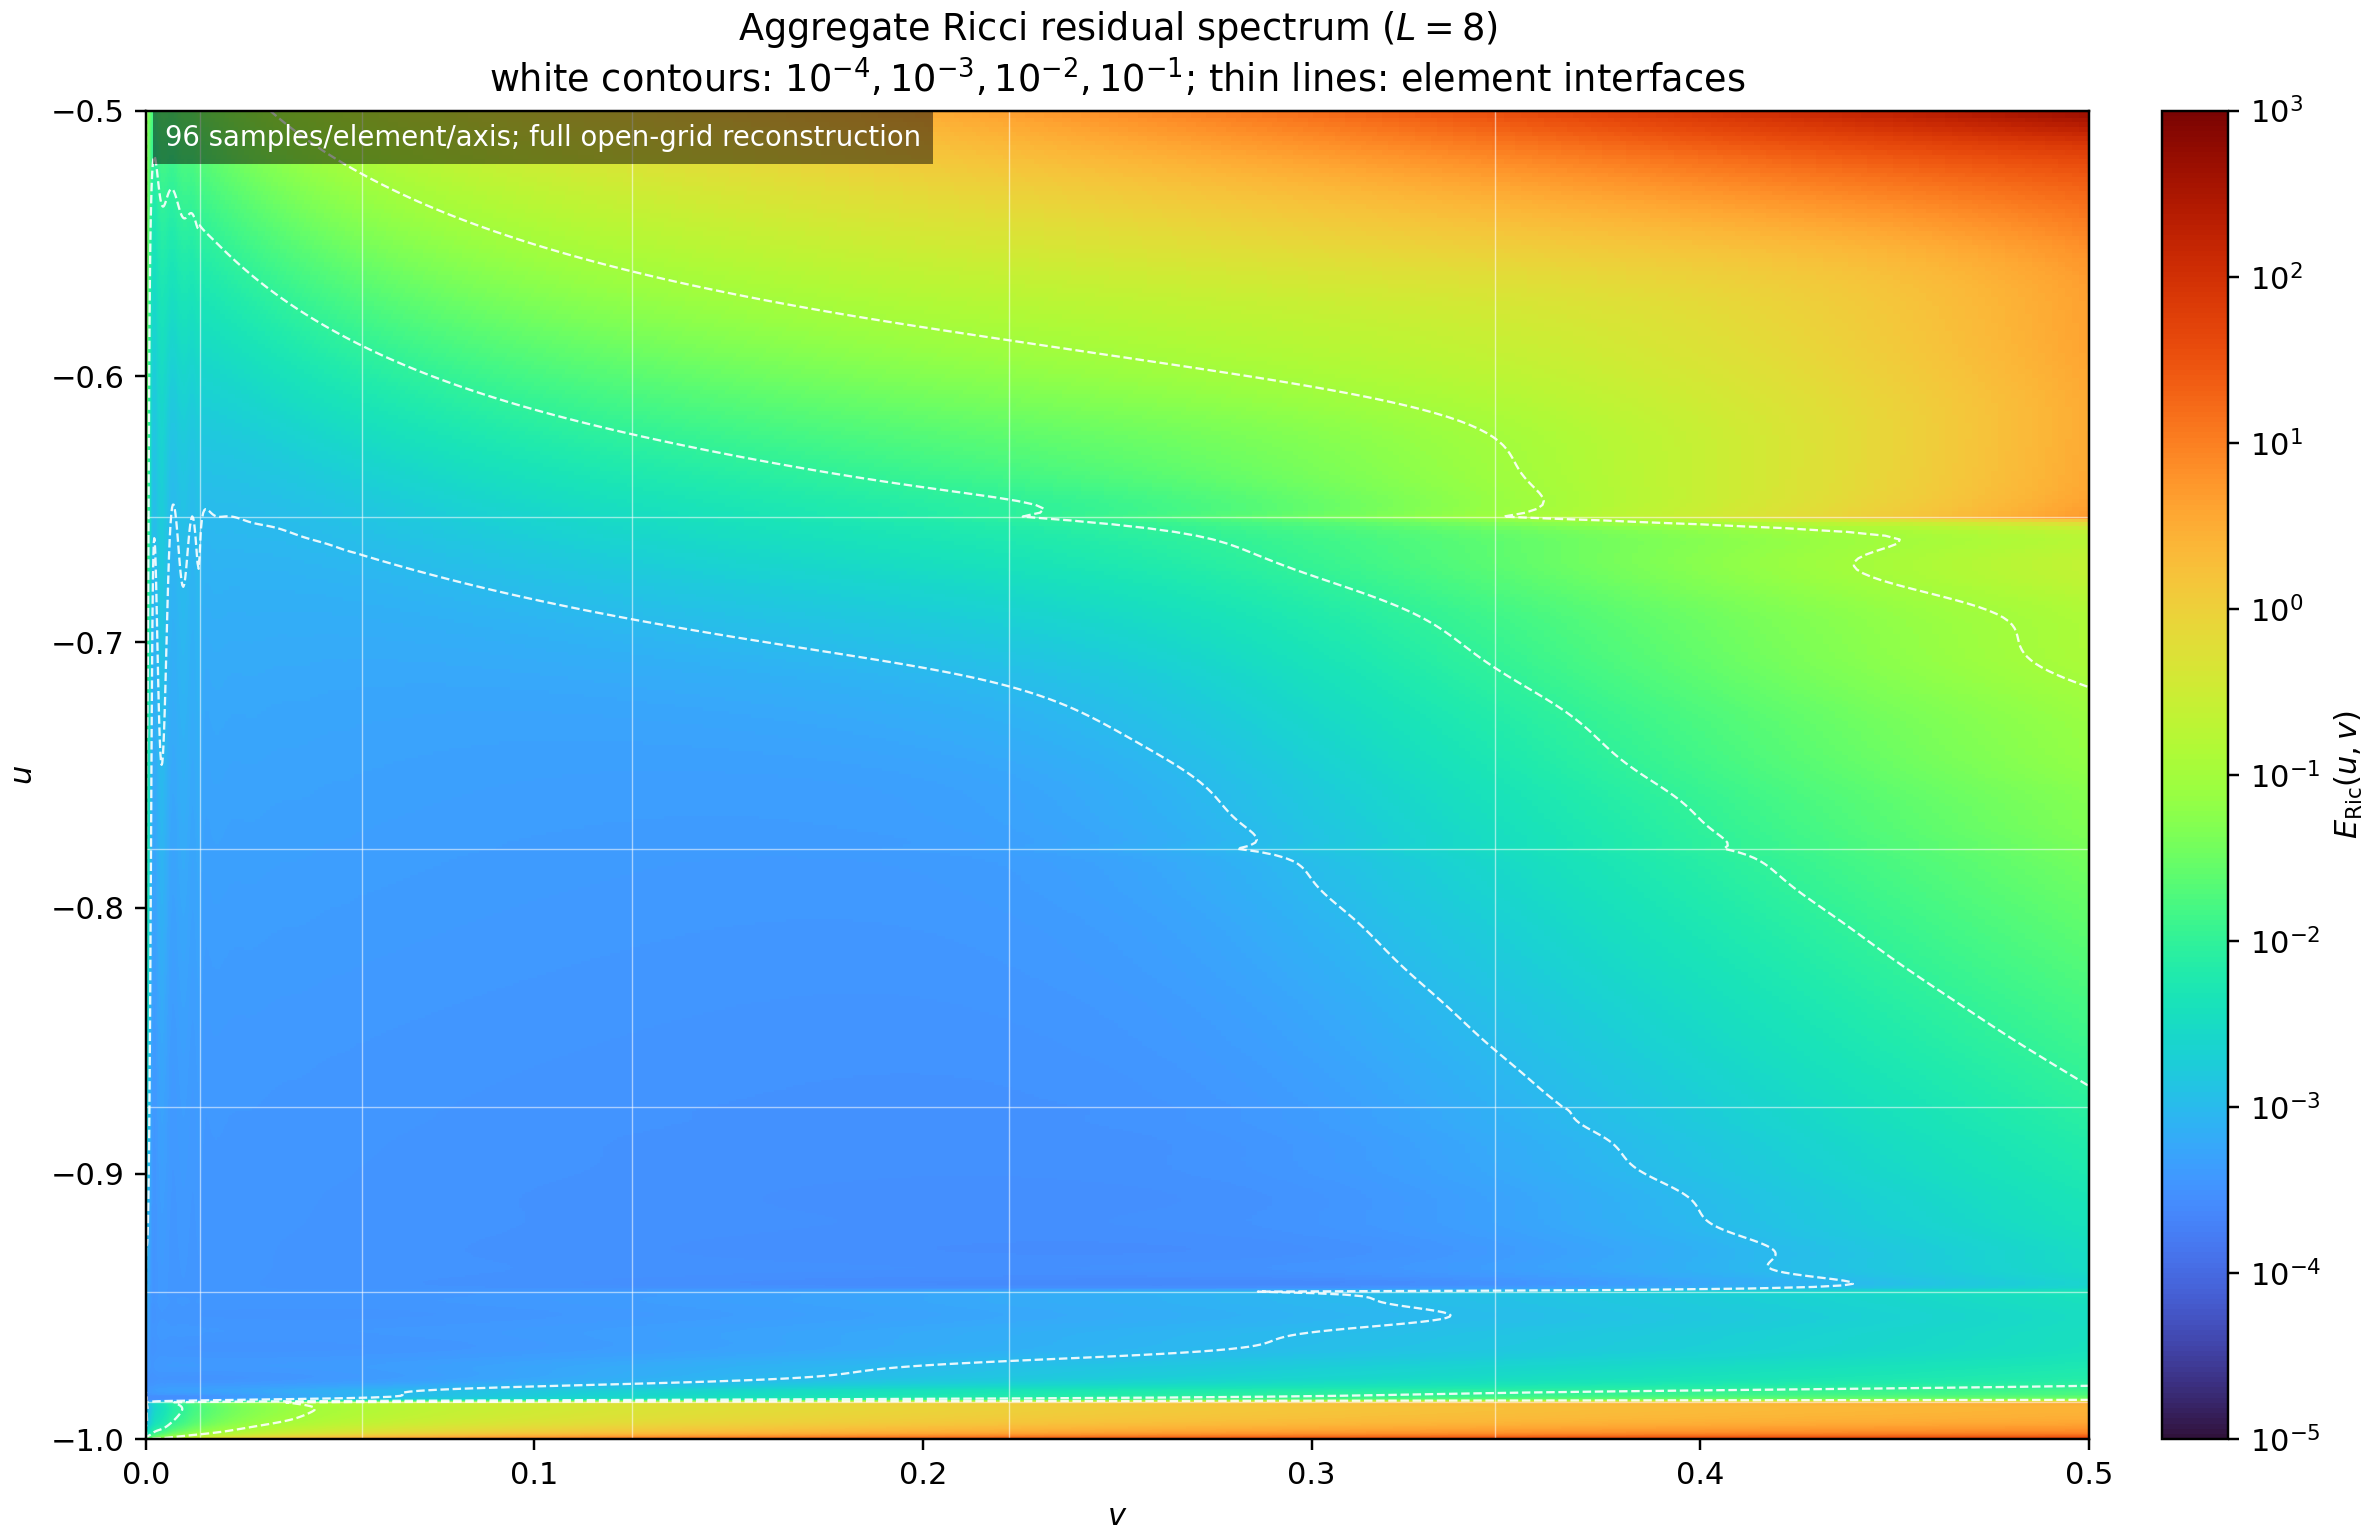
\includegraphics[width=0.8\textwidth]{
    ../experiments/exp05/results/residual-spectrum.png}
  \caption{Spectrum of the aggregate Ricci residual
  $E_{\mathrm{Ric}}(u,v)$.  Colors show the elementwise spectral
  interpolation of $\log_{10}E_{\mathrm{Ric}}$ on the open coordinate
  grid; white contours mark $10^{-4}$, $10^{-3}$, $10^{-2}$, and $10^{-1}$,
  and the thin lines are coordinate-element interfaces.}
  \label{fig:results-exp5-residual-spectrum}
\end{figure}

Figure \ref{fig:results-exp5-residual-spectrum} includes the unprotected
layers of the open grid.  The extreme null-curvature components can diverge
at the initial corner, but they are not differentiated to obtain this
residual.  The large unprotected values instead expose errors in the
first-order differentiation near the fractional-power endpoints and element
interfaces.  They are not used as an interior accuracy statistic; the
protected values are reported in Table~\ref{tab:results-exp5-residual}.

% \clearpage

\section{Results for Einstein Scalar-field Equations}

\section[Conclusion and Outlook]{\hspace{0.4em}Conclusion and Outlook}%
\label{sec:conclusion}

We have developed a first-order Picard iteration for the characteristic
initial value problem for the Einstein vacuum and Einstein--massless-scalar
equations in double-null gauge.  The construction follows the geometric
dependency structure of the equations and combines characteristic constraint
solves with spectral elements in the two null coordinates, pole-free angular
operators, and independent first-order residual audits with separate
metric--connection consistency checks.  This provides a unified
numerical framework for exact benchmarks and for characteristic data with no
explicit interior solution.

The regular exact tests cover vacuum Schwarzschild and Kerr geometries and the
scalar Fisher--JNW family.  Metric errors remain small in regular domains and
across a Schwarzschild horizon.  The Schwarzschild-interior experiment also
identifies the present method's loss of accuracy as the curvature singularity
is approached.  Beyond the explicit families, the vacuum calculations evolve
a strong nonspherical outgoing perturbation and crossed characteristic data
with singular limiting initial curvature.  The Einstein--scalar calculations
further demonstrate
coordinate convergence for nonspherical, low-regularity characteristic data
on the protected numerical region.

The final experiment gives numerical evidence for a trapped region and
reconstructs its apparent horizon.  On the curved characteristic domain, both
angular discretizations identify the section
\begin{equation}
  (u,v)=(-0.4696271025,0.04),
\end{equation}
where the two future null expansions are strictly negative on the entire
sphere.  Eighteen independently reconstructed MOTSs form a sampled
apparent-horizon tube over $0.00441\leq v\leq0.05$.  Coordinate refinement
changes its $v=0.04$ graph by $1.50\times10^{-7}$ in maximum norm, while an
independent higher-angular-band evolution changes its mean location by
$7.80\times10^{-10}$.  The distinction between exact metric errors,
independently evaluated curvature residuals, trapped-section sign tests, and
the graph MOTS equation remains essential when interpreting the experiments.

Three directions are particularly important for future work.  First, the
angular MOTS solve should be extended with adaptive coordinate refinement
toward the singular endpoint and across alternative foliations, thereby
resolving the anisotropic apparent horizon more completely.  Second, varying
the scalar-pulse and anisotropic-perturbation
amplitudes would reveal the threshold for trapping and the dependence of the
first trapped location on the initial data.  Third, improved coordinates,
adaptive refinement, and more robust iteration strategies are needed to
improve the approximation near curvature singularities.  These developments
would extend the present double-null framework from a local numerical
construction toward a more precise study of anisotropic black-hole formation
and singular spacetime geometry.


\section*{Code availability}
The source code, experiment configurations, and instructions for reproducing
the numerical experiments are available at\\
\url{https://github.com/Shengrong-Wu/Numerical-Einstein-Equations}.
% The version associated with this article is identified by release
% \texttt{vX.Y.Z} and commit \texttt{COMMIT-HASH}.

\bibliographystyle{plain}
\bibliography{ref}

\end{document}
